\documentclass[a4paper,11pt,fleqn,dvipsnames,twoside,openany]{memoir} 	% Openright aabner kapitler paa hoejresider (openany begge)

%%%% PACKAGES %%%%

% ¤¤ Oversaettelse og tegnsaetning ¤¤ %
\usepackage[utf8]{inputenc}					% Input-indkodning af tegnsaet (UTF8)
\usepackage[english]{babel}					% Dokumentets sprog
\usepackage[T1]{fontenc}					% Output-indkodning af tegnsaet (T1)
\usepackage{ragged2e,anyfontsize}			% Justering af elementer
\usepackage{fixltx2e}						% Retter forskellige fejl i LaTeX-kernen
																			
% ¤¤ Figurer og tabeller (floats) ¤¤ %
\usepackage{caption}
\usepackage{subcaption}
\usepackage{graphicx} 						% Haandtering af eksterne billeder (JPG, PNG, EPS, PDF)
%\usepackage{eso-pic}						% Tilfoej billedekommandoer paa hver side
%\usepackage{wrapfig}						% Indsaettelse af figurer omsvoebt af tekst. \begin{wrapfigure}{Placering}{Stoerrelse}
\usepackage{multirow}                		% Fletning af raekker og kolonner (\multicolumn og \multirow)
\usepackage{multicol}         	        	% Muliggoer output i spalter
\usepackage{rotating}						% Rotation af tekst med \begin{sideways}...\end{sideways}
\usepackage{colortbl} 						% Farver i tabeller (fx \columncolor og \rowcolor)
\usepackage[table]{xcolor}				 	% Definer farver med \definecolor. Se mere: http://en.wikibooks.org/wiki/LaTeX/Colors
\usepackage{flafter}						% Soerger for at floats ikke optraeder i teksten foer deres reference
\let\newfloat\relax 						% Justering mellem float-pakken og memoir
\usepackage{float}							% Muliggoer eksakt placering af floats, f.eks. \begin{figure}[H]
\usepackage{wrapfig}



% ¤¤ Matematik mm. ¤¤
\usepackage{amsmath,amssymb,stmaryrd} 		% Avancerede matematik-udvidelser
\usepackage{mathtools}						% Andre matematik- og tegnudvidelser
\usepackage{textcomp}                 		% Symbol-udvidelser (f.eks. promille-tegn med \textperthousand )
\usepackage{rsphrase}						% Kemi-pakke til RS-saetninger, f.eks. \rsphrase{R1}
\usepackage[version=3]{mhchem} 				% Kemi-pakke til flot og let notation af formler, f.eks. \ce{Fe2O3}
\usepackage{siunitx}						% Flot og konsistent praesentation af tal og enheder med \si{enhed} og \SI{tal}{enhed}
\sisetup{locale=DE}							% Opsaetning af \SI (DE for komma som decimalseparator) 

% ¤¤ Referencer og kilder ¤¤ %
\usepackage[danish]{varioref}				% Muliggoer bl.a. krydshenvisninger med sidetal (\vref)
\usepackage[square,sort,comma,numbers]{natbib}							% Udvidelse med naturvidenskabelige citationsmodeller
%\usepackage{xr}							% Referencer til eksternt dokument med \externaldocument{<NAVN>}
%\usepackage{glossaries}					% Terminologi- eller symbolliste (se mere i Daleifs Latex-bog)

% ¤¤ Misc. ¤¤ %
\usepackage{lipsum}							% Dummy text \lipsum[..]
\usepackage[shortlabels]{enumitem}			% Muliggoer enkelt konfiguration af lister
\usepackage{pdfpages}						% Goer det muligt at inkludere pdf-dokumenter med kommandoen \includepdf[pages={x-y}]{fil.pdf}	
\pdfoptionpdfminorversion=6					% Muliggoer inkludering af pdf dokumenter, af version 1.6 og hoejere
\pretolerance=2500 							% Justering af afstand mellem ord (hoejt tal, mindre orddeling og mere luft mellem ord)

% Kommentarer og rettelser med \fxnote. Med 'final' i stedet for 'draft' udloeser hver note en error i den faerdige rapport.
\usepackage[footnote,final,english,silent,nomargin]{fixme}		
\usepackage[bottom]{footmisc}

%%%% CUSTOM SETTINGS %%%%

% ¤¤ Marginer ¤¤ %
\setlrmarginsandblock{3.5cm}{2.5cm}{*}		% \setlrmarginsandblock{Indbinding}{Kant}{Ratio}
\setulmarginsandblock{2.5cm}{3.0cm}{*}		% \setulmarginsandblock{Top}{Bund}{Ratio}
\checkandfixthelayout 						% Oversaetter vaerdier til brug for andre pakker

%	¤¤ Afsnitsformatering ¤¤ %
\setlength{\parindent}{0mm}           		% Stoerrelse af indryk
\setlength{\parskip}{3mm}          			% Afstand mellem afsnit ved brug af double Enter
\linespread{1,1}							% Linie afstand

% ¤¤ Litteraturlisten ¤¤ %
%\bibpunct[,]{[}{]}{;}{a}{,}{,} 				% Definerer de 6 parametre ved Harvard henvisning (bl.a. parantestype og seperatortegn)
%\bibliographystyle{bibtex/harvard}			% Udseende af litteraturlisten.
\bibliographystyle{ieeetr}	

% ¤¤ Indholdsfortegnelse ¤¤ %
\setsecnumdepth{subsection}		 			% Dybden af nummerede overkrifter (part/chapter/section/subsection)
\maxsecnumdepth{subsection}					% Dokumentklassens graense for nummereringsdybde
\settocdepth{section} 					% Dybden af indholdsfortegnelsen

% ¤¤ Lister ¤¤ %
\setlist{
  topsep=0pt,								% Vertikal afstand mellem tekst og listen
  itemsep=-1ex,								% Vertikal afstand mellem items
} 

% ¤¤ Visuelle referencer ¤¤ %
\usepackage[colorlinks]{hyperref}			% Danner klikbare referencer (hyperlinks) i dokumentet.
\hypersetup{colorlinks = true,				% Opsaetning af farvede hyperlinks (interne links, citeringer og URL)
    linkcolor = black,
    citecolor = black,
    urlcolor = black
}

% ¤¤ Opsaetning af figur- og tabeltekst ¤¤ %
\captionnamefont{\small\bfseries\itshape}	% Opsaetning af tekstdelen ('Figur' eller 'Tabel')
\captiontitlefont{\small}					% Opsaetning af nummerering
\captiondelim{. }							% Seperator mellem nummerering og figurtekst
\hangcaption								% Venstrejusterer flere-liniers figurtekst under hinanden
%\captionwidth{\linewidth}					% Bredden af figurteksten
\setlength{\belowcaptionskip}{10pt}			% Afstand under figurteksten
		
% ¤¤ Navngivning ¤¤ %
\addto\captionsdanish{
	\renewcommand\appendixname{Appendiks}
	\renewcommand\contentsname{Indholdsfortegnelse}	
	\renewcommand\appendixpagename{Appendiks}
	\renewcommand\appendixtocname{Appendiks}
	\renewcommand\cftchaptername{\chaptername~}				% Skriver "Kapitel" foran kapitlerne i indholdsfortegnelsen
	\renewcommand\cftappendixname{\appendixname~}			% Skriver "Appendiks" foran appendiks i indholdsfortegnelsen
}

% ¤¤ Kapiteludssende ¤¤ %
\definecolor{numbercolor}{gray}{0.7}		% Definerer en farve til brug til kapiteludseende
\newif\ifchapternonum

\makechapterstyle{E4}{					% Definerer kapiteludseende frem til ...
  \renewcommand\beforechapskip{0pt}
  \renewcommand\printchaptername{}
  \renewcommand\printchapternum{}
  \renewcommand\printchapternonum{\chapternonumtrue}
  \renewcommand\chaptitlefont{\fontfamily{pbk}\fontseries{db}\fontshape{n}\fontsize{25}{35}\selectfont\raggedleft}
  \renewcommand\chapnumfont{\fontfamily{pbk}\fontseries{m}\fontshape{n}\fontsize{1in}{0in}\selectfont\color{numbercolor}}
  \renewcommand\printchaptertitle[1]{%
    \noindent
    \ifchapternonum
    \begin{tabularx}{\textwidth}{X}
    {\let\\\newline\chaptitlefont ##1\par} 
    \end{tabularx}
    \par\vskip-2.5mm\hrule
    \else
    \begin{tabularx}{\textwidth}{Xl}
    {\parbox[b]{\linewidth}{\chaptitlefont ##1}} & \raisebox{-15pt}{\chapnumfont \thechapter}
    \end{tabularx}
    \par\vskip2mm\hrule
    \fi
  }
}											% ... her

\chapterstyle{E4}						% Valg af kapiteludseende - Google 'memoir chapter styles' for alternativer

% ¤¤ Sidehoved ¤¤ %

\makepagestyle{IHA}							% Definerer sidehoved og sidefod udseende frem til ...
\makepsmarks{IHA}{%
	\createmark{chapter}{left}{shownumber}{}{. \ }
	\createmark{section}{right}{shownumber}{}{. \ }
	\createplainmark{toc}{both}{\contentsname}
	\createplainmark{lof}{both}{\listfigurename}
	\createplainmark{lot}{both}{\listtablename}
	\createplainmark{bib}{both}{\bibname}
	\createplainmark{index}{both}{\indexname}
	\createplainmark{glossary}{both}{\glossaryname}
}
\nouppercaseheads											% Ingen Caps oenskes

\makeevenhead{IHA}{\leftmark}{}{Ingeniørhøjskolen i Aarhus}								% Definerer lige siders sidehoved (\makeevenhead{Navn}{Venstre}{Center}{Hoejre})
\makeoddhead{IHA}{\leftmark}{}{Ingeniørhøjskolen i Aarhus}		% Definerer ulige siders sidehoved (\makeoddhead{Navn}{Venstre}{Center}{Hoejre})
\makeevenfoot{IHA}{}{\thepage}{}								% Definerer lige siders sidefod (\makeevenfoot{Navn}{Venstre}{Center}{Hoejre})
\makeoddfoot{IHA}{}{\thepage}{}									% Definerer ulige siders sidefod (\makeoddfoot{Navn}{Venstre}{Center}{Hoejre})
\makeheadrule{IHA}{\textwidth}{0.5pt}							% Tilfoejer en streg under sidehovedets indhold
\makefootrule{IHA}{\textwidth}{0.5pt}{1mm}						% Tilfoejer en streg under sidefodens indhold

\copypagestyle{IHAchap}{IHA}								% Sidehoved for kapitelsider defineres som standardsider, men med blank sidehoved
\makeoddhead{IHAchap}{}{}{}
\makeevenhead{IHAchap}{}{}{}
\makeheadrule{IHAchap}{\textwidth}{0pt}
\makefootrule{IHAchap}{\textwidth}{0.5pt}{1mm}						% Tilfoejer en streg under sidefodens indhold
\aliaspagestyle{chapter}{IHAchap}							% Den ny style vaelges til at gaelde for chapters
															% ... her
															
\pagestyle{IHA}												% Valg af sidehoved og sidefod


%%%% CUSTOM COMMANDS %%%%

% ¤¤ Billede hack ¤¤ %
\newcommand{\figur}[4]{
		\begin{figure}[H] \centering
			\includegraphics[width=#1\textwidth]{billeder/#2}
			\caption{#3}\label{#4}
		\end{figure} 
}

% ¤¤ Tab hack ¤¤ %
\newcommand{\tab}[1]{\hspace{.2\textwidth}\rlap{#1}}

% ¤¤ Specielle tegn ¤¤ %
\newcommand{\grader}{^{\circ}\text{C}}
\newcommand{\gr}{^{\circ}}
\newcommand{\g}{\cdot}


%%%% ORDDELING %%%%

\hyphenation{}

%%%% FARVER %%%%
\definecolor{light-gray}{gray}{0.95}

%----------------------------------------------------------------------------------------
%	TITLE SECTION
%----------------------------------------------------------------------------------------

\title{\vspace{-15mm}\fontsize{24pt}{10pt}\selectfont\textbf{Robot Project}} % Article title

\author{
\large
\textsc{Rune A. Heick, René Arendt Sørensen \& Nicolai Glud}\\[2mm] % Your name
\normalsize Aarhus University, Department of Engineering \\ % Your institution
\vspace{-5mm}
}
\date{}

%----------------------------------------------------------------------------------------

\begin{document}
\setlength{\abovedisplayskip}{1cm}
\setlength{\belowdisplayskip}{.8cm}
\maketitle % Insert title

\newpage
%----------------------------------------------------------------------------------------
%	ABSTRACT
%----------------------------------------------------------------------------------------

\begin{abstract}
The Content of this paper seeks to present the knowledge gained throughout the AI in Robotics and kalman filters reading course from Aarhus University, department of engineering. 
\end{abstract}
\tableofcontents

%----------------------------------------------------------------------------------------
%	ARTICLE CONTENTS
%----------------------------------------------------------------------------------------

%\begin{multicols}{2} % Two-column layout throughout the main article text
\chapter{Introduction}
The goal of this report is researching how to implement AI in Robotics. The knowledge required for this is acquired from the Udacity course "Artificial Intelligence for Robotics"\cite{AIROK}. The Probabilistic Robots will be used to supplement the knowledge from the Udacity course\cite{thrun2005probabilistic}.

The overall purpose of the course can be described as these points:
\begin{itemize}
\item Define and explain concepts, methods and technologies relating to the chosen subject area.
\item Give an account of research articles relevant to the subject area.
\item Account for the status and application of the subject area.
\item Prepare a report and an oral presentation on the subject area.
\end{itemize}

To fulfil these points this report will be split into two parts, theory and project. The theory will seek to provide an insight into the gained theoretically knowledge about artificial intelligence in robots and kalman filters.
The project part will entail the gained knowledge of implementing the theory in a moving robot.
%------------------------------------------------
% chapter theory
\chapter{Theory}
\section{Localisation}
Localisation is the act of a robot finding out where it is. GPS systems are often used to do this in cases where precision is not critical, e.g. GPS navigation. If precision is critical, e.g. for a robot to drive past obstacles without hitting them, GPS is too imprecise. Other techniques must then be used. To do this, robots often have sensors, such as sonars, LIDARs or cameras. 
The localisation algorithms consists of two main parts, movement and measurement. Movement is imprecise, often because of the mechanical system. Measurements contributes with new knowledge and is therefore the part that narrows the decision, of where the robot is, in. The measurements is often also noisy, but usually less noisy than the movements.
Another important thing in localisation is probability. What is the probability of being in a certain position, given the measurement? To calculate this, Bayes rule is used.
\begin{equation}
p(x|z) = \frac{p(z|x)\cdot p(x)}{p(z)}
\end{equation}
Where $\frac{1}{p(z)}$ is the normalizing factor $\eta$.
\begin{equation}
\eta = \frac{1}{p(z)} = \frac{1}{\sum(p(z|x)\cdot p(x))}
\end{equation}
This gives us the expression:
\begin{equation}
p(x|z) = \eta \cdot p(z|x)\cdot p(x)
\end{equation}

\textbf{Eksample:}\\
A robot is in one of the grids in the map. It can detect if it is in a red or green grid. 
\begin{figure}[H]

\includegraphics[scale=1]{billeder/Localisation01.png}
\caption{The map in which the robot lives}
\end{figure}
If the robot is in a green grid, it detects correctly with 75\% chance. If it is in a red grid, it detects correctly with 90\% chance.
If the robot detects green, what is the probability that it is in a green or a red grid?\\
$z = green$\\
$\eta = \frac{1}{sum(p(z|x)\cdot p(x))} = \frac{1}{0.75 \cdot \frac{3}{5} + 0.1 \cdot 2/5} = 2.04$\\\\
$x = green$\\
$p(x) = \frac{3}{5}$\\
$p(x \mid z) = \eta \cdot p(z|x)\cdot p(x) = 2.04 \cdot 0.75 \cdot \frac{3}{5} = 0.918 = 91.8\%$\\\\
$x = red$\\
$p(x) = \frac{2}{5}$\\
$p(x \mid z) = \eta \cdot p(z|x)\cdot p(x) = 2.04 \cdot 0.1 \cdot \frac{2}{5} = 0.082 = 8.2\%$

\subsection{Markov Localisation}
% Localisation_MarkovLocalisation
The purpose of Markov Localisation is to estimate where the robot is located, given its measurements, movements and a map describing the world in which the robot is placed.
Lets say the robot can move along a wall and sense whether if there is a door next to it or not. We place the robot in a world with a wall with 3 doors.
The estimation of the localisation of the robot is called belief and is the probability of being in a given location, given the previous act. At the beginning, the robot will not know where it is, and therefore it will have a uniformly distributed belief.\\ 
Then the robot takes a measurement, and let's say that it measures a door. Now the new belief is the former belief multiplied with the probability of the measurement z given the position x. 
\begin{equation}
bel'(x) = bel(x) \cdot p(z|x)
\label{ML_eq1}
\end{equation}
After this the robot moves. A movement is often noisy and therefore the precision of the belief will fall. This is illustrated by convolving the belief with the motion model. The motion model consists of a mean $\mu$, representing the noise free movement, and a standard deviation $\sigma$, representing the noise. The result of this step can be seen in \ref{ML_fig1:sub3}.
\begin{equation}
bel'(x) = bel(x) \ast norm(\mu,\sigma)
\label{ML_eq2}
\end{equation}
These two steps are now repeated the rest of the lifetime of the robot. Every time the robot senses, it gets more certain of where it is and every time it moves it gets more uncertain. In figure \ref{ML_fig1} two iterations are shown.

\begin{figure}[H]
\centering

\begin{subfigure}[b]{.8\textwidth}
  \centering
  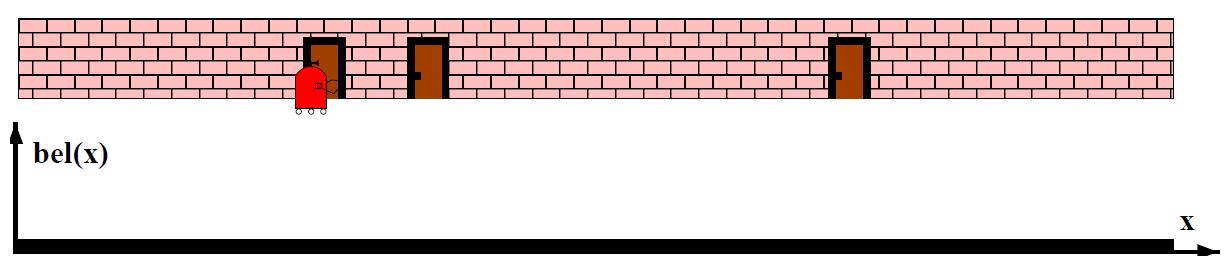
\includegraphics[width=1\linewidth]{billeder/MarkovLocalisation01.png}
  \caption{Initial belief is uniformly distributed.}
  \label{ML_fig1:sub1}
\end{subfigure}%

\begin{subfigure}[b]{.8\textwidth}
  \centering
  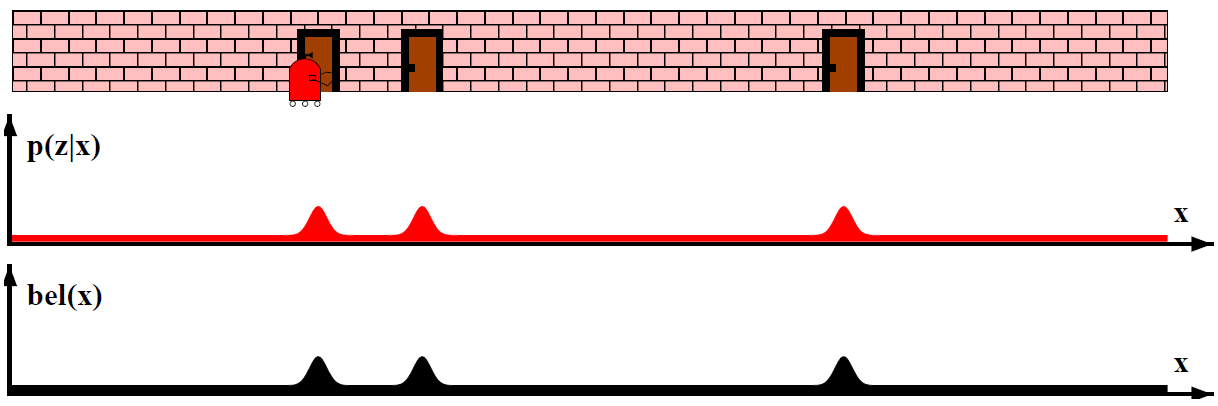
\includegraphics[width=1\linewidth]{billeder/MarkovLocalisation02.png}
  \caption{Measurement and result of belief multiplied with measurement.}
  \label{ML_fig1:sub2}
\end{subfigure}

\begin{subfigure}[b]{.8\textwidth}
  \centering
  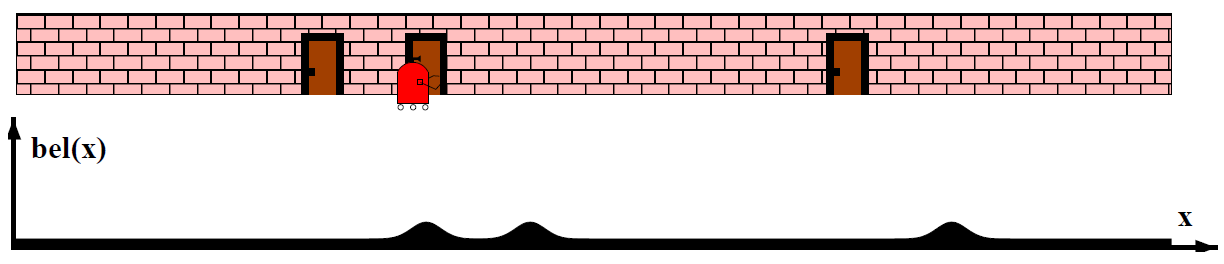
\includegraphics[width=1\linewidth]{billeder/MarkovLocalisation03.png}
  \caption{Movement of robot and belief. Noise makes the belief after the movement more uncertain.}
  \label{ML_fig1:sub3}
\end{subfigure}%

\begin{subfigure}[b]{.8\textwidth}
  \centering
  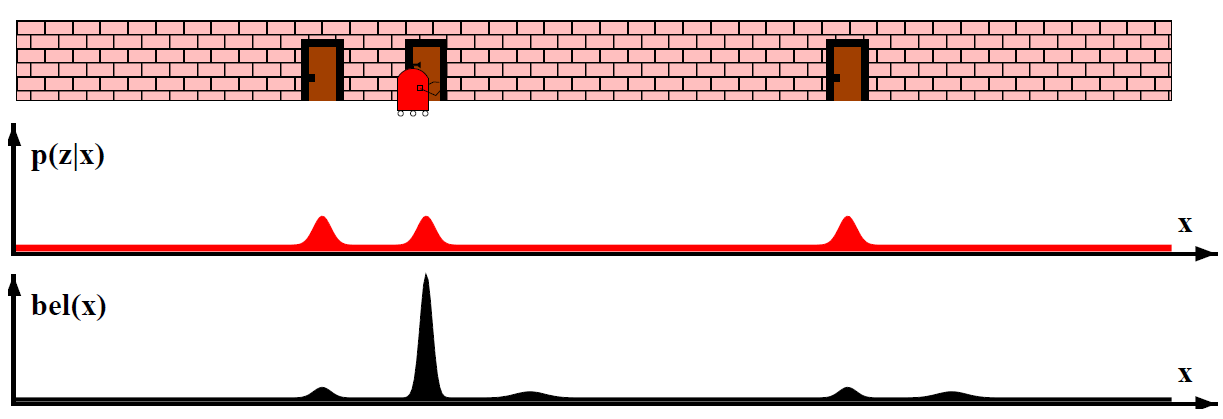
\includegraphics[width=1\linewidth]{billeder/MarkovLocalisation04.png}
  \caption{Measurement and result of belief multiplied with measurement.}
  \label{ML_fig1:sub4}
\end{subfigure}

\begin{subfigure}[b]{.8\textwidth}
  \centering
  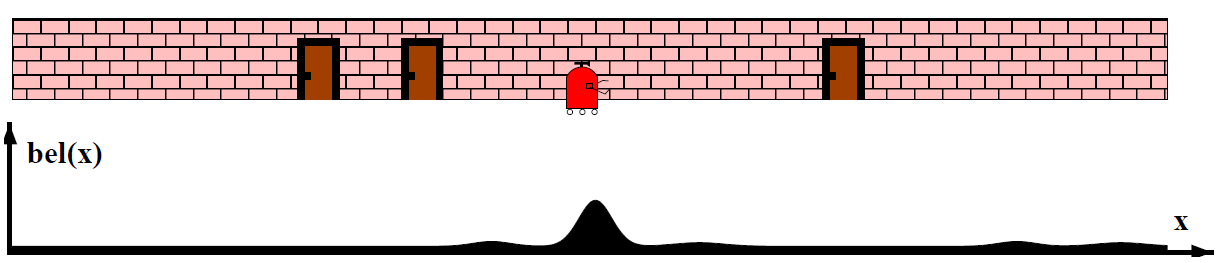
\includegraphics[width=1\linewidth]{billeder/MarkovLocalisation05.png}
  \caption{Movement of robot and belief. Noise makes the belief after the movement more uncertain.}
  \label{ML_fig1:sub5}
\end{subfigure}

\caption{Markov Localisation illustrated. \citep{thrun2005probabilistic}}
\label{ML_fig1}
\end{figure}

The algorithm for Markov Localisation is as follows:\\
1:\quad \textbf{Algorithm MarkovLocalization(}$bel(x_{t-1}),u_t,z_t,m$\textbf{):}\\
2:\quad \quad $for\,all\,x_t\,do$\\
3:\quad \qquad $\overline{bel}(x_t) = \int p(x_t|u_t,x_{t-1},m)\cdot bel(x_{t-1}) dx$\\
4:\quad \qquad $bel(x_t) = \eta p(z_t|x_t,m)\cdot \overline{bel}(x_t)$\\
5:\quad \quad $endfor$\\
6:\quad \quad $return\,bel(x_t)$

What happens is that after a move, $u_t$, and a measurement, $z_t$, has been taken, the algorithm is called. First it calculates the belief after the movement, and then it calculates the belief after the measurement. It does this for all possible places, $x_t$, in the map, $m$. This corresponds to the combinations of (a and b) or (c and d) in figure \ref{ML_fig1}.

\subsection{Kalman Filter}
The kalman filter is a method for sensor fusion. It is capable of taking two or more measurements and fuse together to one optimal guess of the true value. It does this by looking at the current measurement and comparing it with a predicted value. The predicted value is often a combination of the previous value combined with the changed done since the last measurement. 

The kalman filter has some limitations. One of them is that it assume that all noise in the system is Gaussian distributed, which is not always the case. Another is that it always gives only one guess on the value, which is optimal for a lot of systems but is not especially preferable in localisation. The last one is that it assumes that there is a linear relationship between all measurements and the value we are trying to estimate. 

Much like the Markov localisation the kalman filter have a measurement step, then it does some movement and predict the new value. This is done in a never ending continues process. 
\begin{figure}[H]
\centering
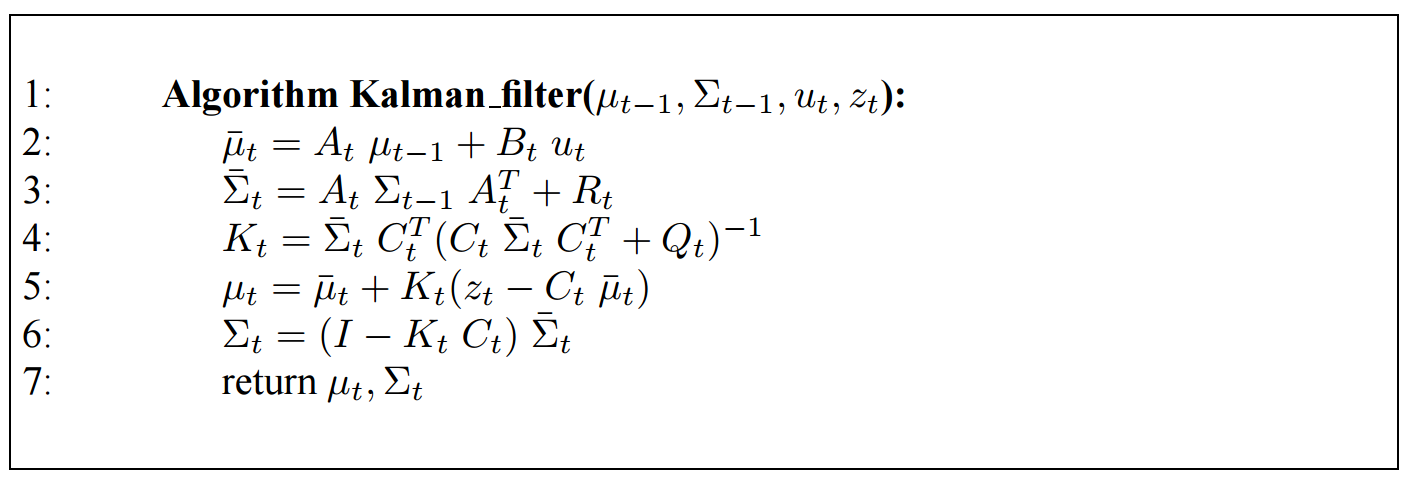
\includegraphics[width=1\textwidth]{billeder/KalmanFilter.png}
\caption{Kalman Filter algorithm}
\label{fig:kalmanfilter}
\end{figure}
If we look at the math, we can see that this can be done in a few steps. looking at the equations of the kalman filter we normally call 2-3 for the prediction step and 4-7 for the measurement step. 
\subsubsection{Prediction Step}
Looking at the equations in the prediction step (\ref{Pre1}, \ref{Pre2}).
\begin{gather}
\overline{\mu}_t = A_t \mu_{t-1} + B_t u_t
\label{Pre1}\\
\overline{\Sigma}_t = A_t \Sigma_{t-1} A^{\intercal}_t+ R_t
\label{Pre2}
\end{gather}
There are 2 conversion matrices $A$, $B$ and a measurement/input matrix $u$. The matrix $A$ must transform the last best estimate to the current domain. e.g. if we are trying to predict how far down a bungee jumper have fallen then the $A$ matrix must add the distance the gravity would have pulled him down since the last estimate $\mu_{t-1}$. We call this the static influence, since it is the change in the system if we do not interfere. The input matrix $u$ is the change we put in to the system since the last prediction. Lets say that we can increase or decrease the bungee jumpers air resistance. The $u$ matrix will contain the information about the change in air resistance. The $B$ matrix will convert the input matrix to the desired domain. For the bungee jumper it will convert air resistance to a fall distance. We call this the dynamic influence.
The last matrix $R$ is the noise, expressed as the covariance, of the input matrix $u$. This is to inform the system about the certainty of the input. 

As previously mentioned this dictates that there exists a linear conversion from the static and dynamic influences in relation to the the previous state to the new state. 
\subsubsection{Measurement Step}
Looking at the equations in the measurement step (\ref{Mes1}, \ref{Mes2} , \ref{Mes3}).
\begin{gather}
K_t = \overline{\Sigma}_t C^{\intercal}_t ( C_t \overline{\Sigma}_t C^{\intercal}_t + Q_t ) ^{-1} 
\label{Mes1} \\
\mu_{t} = \overline{\mu}_t +K_t (z_t-C_t\overline{\mu}_t) 
\label{Mes2} \\
\Sigma_t = (I-K_t C_t) \overline{\Sigma}_t 
\label{Mes3}
\end{gather}
The measurement step takes the predicted value $\overline{\mu}_t$, $\overline{\Sigma}_t$ and uses the measurement to fix the error in the prediction introduced by the noise. The measurement vector $z_t$ contains the measurement. For the bungee jumper it could be the tension in the bungee line. The conversion matrix $C_t$ convert the measurement to the value domain. So it takes the tension and convert to a distance. The $Q_t$ matrix is our measurement noise, expressed as the covariance.

By calculating the Kalman gain $K_t$ we get a kind of believe on the measurement, that decides how much we are able to affect the predicted value with information obtained from the measurement. 

After we have corrected the prediction, we have the best possible guess of the true value, or the true distance in the bungee case. 
\subsubsection{Graphical}
Looking at the bungee example, this can also be graphically shown. On figure \ref{bungeeFig} we see the bungee problem. 
\begin{figure}[H]
\centering
\includegraphics[width=1\textwidth]{billeder/Bungee.jpg}
\caption{The bungee problem}
\label{bungeeFig}
\end{figure}
First we see a the prediction step which have a very high uncertainty as shown with a Gaussian with a big variance. After this we make a measurement, as show in the second graph. we now use the kalman filter to estimate the best guess, based on the prediction and the measurement. 

We can see this as optimal fusion of our prediction information and our measurement information. 
\subsubsection{Kalman Filters In Robotics}
Like in the bungee example where the position of the bungee jumper was found. A robot can be located in a known map. 
But this is not the only use of a kalman filters in robotics.\\
Kalman filters are often used to fuse multiple sensor readings to one optimal guess, and to discover hidden variables. A hidden variable is a property that can not be directly measured, but have a relation to the measured data. lets say you can measure the location of a robot. Then the hidden variable can be the robots speed since the speed can be found looking at different locations over time. By using a kalman filter it is possible to estimate the speed very precise. \\
Since the kalman filter is uni-model, which mean that it only can give one guess of the location, other techniques, like particle filters and Markov localisation which gives multiple candidate locations, are often preferred. 
\subsubsection{Extended Kalman Filter}
One of the big limitations of the kalman filter is the requirement that dictates that there must be a linear relationship between measurements or input and the value domain. 

This limitation is removed in the extended kalman filter. This is done by replacing the linear conversion matrices $A$, $B$ and $C$ with the none linear functions $g(u_t, \mu_{t-1})$ and $h(\overline{\mu}_t)$.\\

Since the kalman filter basically exploits the principle of a Gaussian converted with a linear transformation still is a Gaussian. Introducing the non linear functions brakes the filter. To fix this the extended kalman filter utilize a method called first order Taylor expansion. Taylor expansion construct a linear approximation to a function, in a given point. This is done by using the partial derivative of the function in the point. We create the partial derivative matrices $G$ and $H$.
\begin{equation}
G = \frac{\partial g(u_t, \mu_{t-1})}{\partial \mu_{t-1}} \\ H = \frac{\partial h(\overline{\mu}_t)}{\partial \overline{\mu}}
\end{equation}
We can now use this in the regular kalman filter to obtain the extended kalman filter.
\begin{figure}[H]
\centering
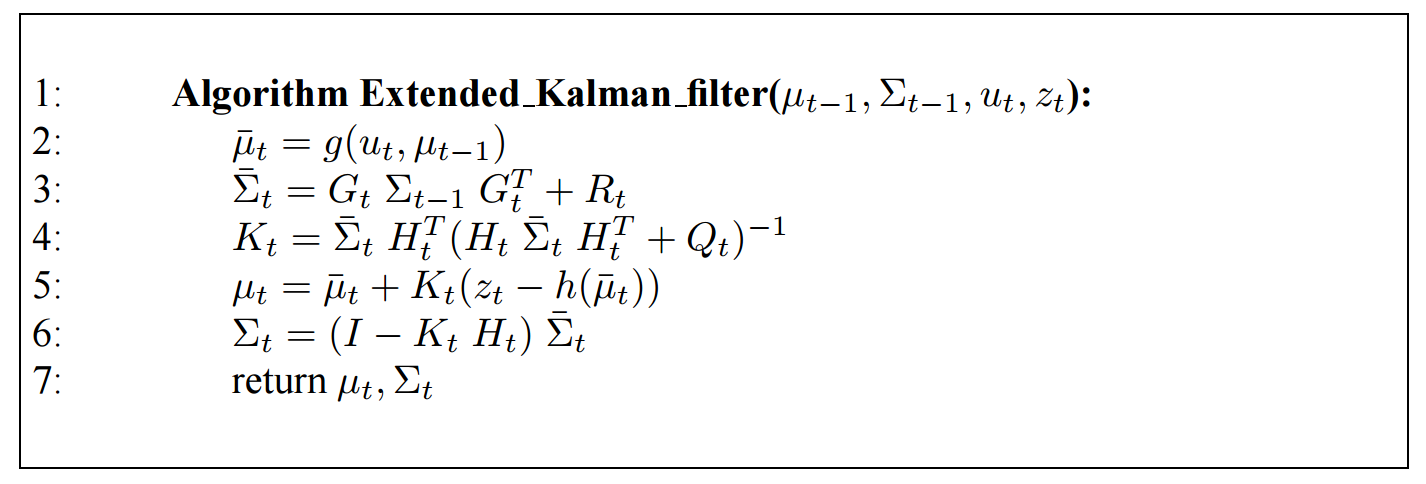
\includegraphics[scale=0.51]{billeder/EKF.png}
\caption{Extended Kalman Filter algorithm}
\end{figure}
It has been shown that this type of kalman filter is far better in practice than the regular kalman filter if the variance of prediction and measurement is small. If this is not the case the linearisation introduces additional noise. This is due to the error between the linearisation and the true function. The greater the variance the greater impact it has.  



\subsection{Particle Filter}
The particle filter is a different kind of filter, since it uses a discrete method for finding the robots location, in contrast to the continuously methods previously discuses. \\
The method is multi-model, which means that more than one location candidate can be found. This is a very popular technique for localisation, since it is simple to understand and implement. 
\\
\\
Like the other filters, the particle filter does also require the map to be known, and we must be able to predict how all measurements will look in any given location. 

The particle filter can also be seen as having a prediction step and a measurement step. Before we start the measurement-prediction loop, we first select a number $M$ of particles $X$ to use in the filter. Then we place all the $M$ particles at random locations. 

\subsubsection{Prediction Step}
After the robot have moved with a motion $u_t$, we move all the particles with the same motion. On this motion we add some random noise $w_t$. If one of the particles was exactly at the robot location before we moved it, and the noise we put on the particle was the exact same as on the real robot, the new particle location would still be the same as the robot.  

\subsubsection{Measurement Step}
First we take the measurement from the real robot $z_t$. Then we compare it to all of the $M$ particles and calculate the probability off the location of the real robot is the same as for the particle. This is done by comparing the measurement $z_t$, with the measurement that would have been at the particle location.
At this process it is important to assume that there is noise on the measurements. If we assume that the sensor is to precise we risk giving particles that are close to the real location a low probability, which is not desirable.\\\\
When we have all the probabilities for the particles $Prob_t$, we are doing resampling. The aim of resampling is to get a new set of $M$ new particles. The locations of the new particles must be randomly drawn from the old particle set whit a distribution that matches the $Prob_t$ distribution. This means that a lot of the new particles are at the locations with high probability, where only a few or none is at locations with low probability.\\ 
\\
After the resampling we continue with the prediction step, and so one. 

\subsubsection{The Algorithm}
Over time particles with at bad locations will die, and more will search the area around feasible locations. The predict - measurement steps can also be expressed as pseudo code as seen below: 

\begin{figure}[H]
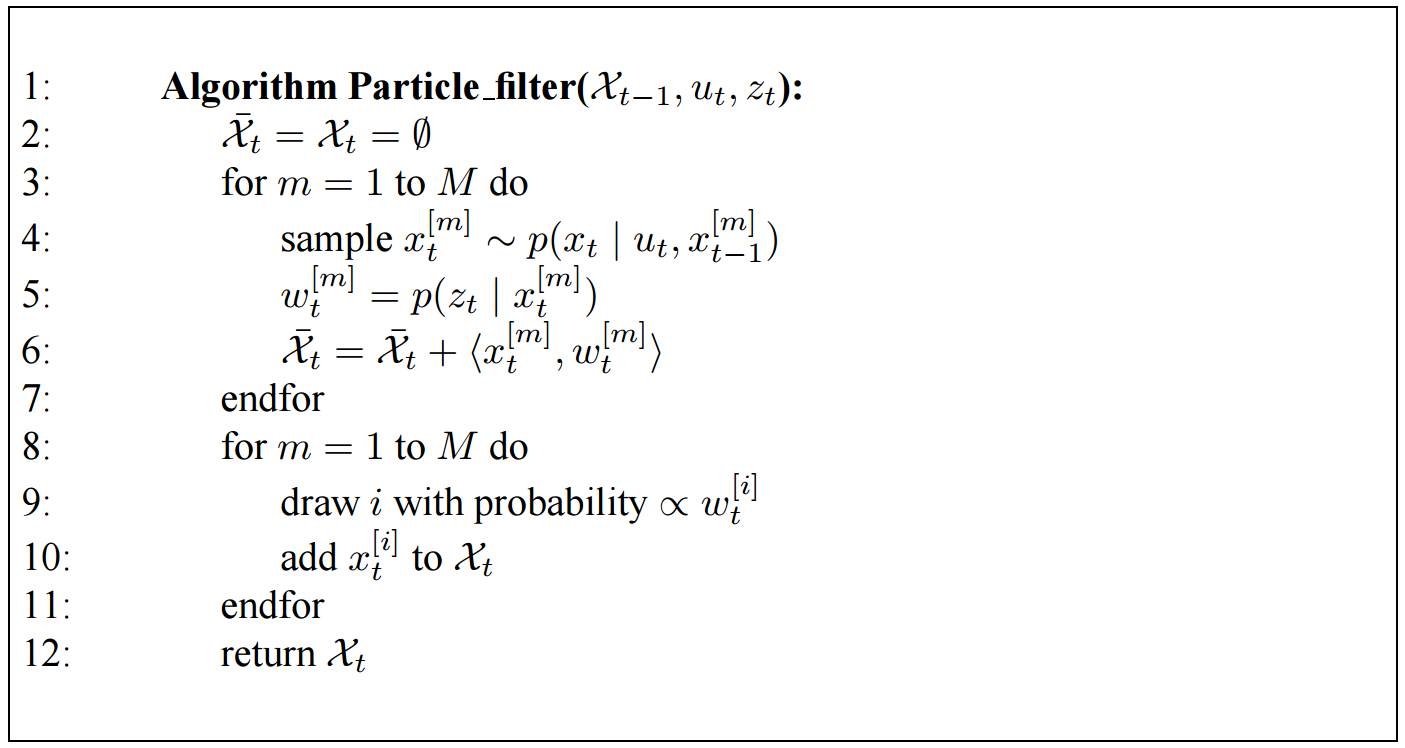
\includegraphics[scale=0.51]{billeder/ParticleFilter.png}
\end{figure}

This process runs continuously, and will over time converge to zero or one single location.

\subsubsection{Particle Filters Considerations}
A series of scenarios must be considered when using particle filters. One is the scenario where there is not placed a particle close to the real robot or all the particles around it dies. This will make the particle filter coverage around a wrong location or no location. There are several techniques tackling this problem. One easy simple solution is to look at probability and see if there is at least one good candidate. If this is not the case the filter should be reset. 
\\\\
One other problem happens if the world is symmetric, this means that every measurement have multiple feasible locations, and when moved previously feasible locations still appearers equally likely. If this is the case it is impossible to know the true location. This is can also in extreme cases be a problem if the world is only partially symmetric, since all the true particles can die, and only the wrong survive. When we now enter a asymmetric area all the wrong will die, and we have no particles left. This can be fixed by either resetting the filter, or by a technique where you all ways randomly spread out the worst $5\%$ of you particles. 
\\\\
Also a balance must be found with the number of particles and the map size. The more particles the better the filter, but it will also drastically increase the calculation time. 

%------------------------------------------------
\section{Search and Planning}
\lipsum[7] % Dummy text

%------------------------------------------------
\section{Control}
\subsection{Smoothing}
The purpose of smoothing is to create a new path without very sharp turns. The new path is also more like a continuous function and very likely also shorter in length. It is important to observe the smoothed path in order to find out whether the new path will move the robot into objects placed along the route.\\
To smooth out the path we use an algorithm that retains the start and goal while smoothing points in between. The first step is to initialise $y_i = x_i$ and then optimise equation \ref{eq:optimisesmooth} with respect to equations \ref{eq:equationsforsmooth1} and \ref{eq:equationsforsmooth2}.
\begin{gather}
minimise (x_i - y_i )^2 + \alpha(y_i - y_{i+1})^2
\label{eq:optimisesmooth} \\
y_i = y_i + \alpha(x_i - y_i)
\label{eq:equationsforsmooth1} \\
y_i = y_i + \beta(y_{i+1} + y_{i-1}-2y_i)
\label{eq:equationsforsmooth2}
\end{gather}
With $0\leq\alpha\leq1$ being how much we want to retain from the original path and $0\leq\beta\leq1$ being how much we want the path smoothed. This will results in something that looks like figure \ref{fig:pathsmooth}. The green circle shows the extend of the equations being optimised at three points.
\begin{figure}[H]
\centering
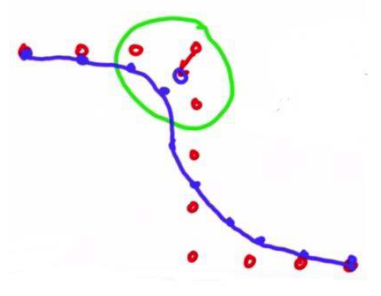
\includegraphics[width=0.4\textwidth]{billeder/pathsmoothed1}
\caption{Original points and a smoothed path}
\label{fig:pathsmooth}
\end{figure}

\subsection{PID Control}
PID is short for Proportional Integral Derivative. These three parts can be seen in equation \ref{eq:pid1}. Where $e(t) = u(t) - y(t)$, $u(t)$ is the control input, $x(t)$ is the input to the motor and $y(t)$ is the output from the motor as an example.
\begin{equation}
x(t) = K_p e(t) + K_i \int^t_0 e(\tau)d\tau + K_d\dfrac{de(t)}{dt}
\label{eq:pid1}
\end{equation}
Each part of the PID controller has a function. The P controller as seen in figure \ref{fig:pcontrol} has the responsibility of reducing the rise time and decreasing the steady-state error. An overshoot appears with larger $K_p$ values. $K_p$ is analogous to a gain.
\begin{figure}[H]
\centering
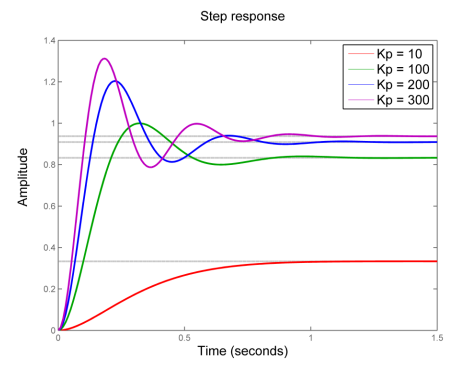
\includegraphics[width=0.5\textwidth]{billeder/pcontrol}
\caption{P Controller with different $K_p$ values}
\label{fig:pcontrol}
\end{figure}
The D controller is used along with the P controller to reduce the overshoot and the settling time. The D controller uses the slope of the function to reduce the error. This is seen in figure \ref{fig:pdcontrol}.
\begin{figure}[H]
\centering
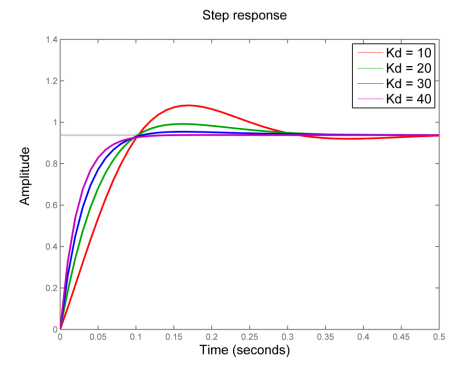
\includegraphics[width=0.5\textwidth]{billeder/pdcontrol}
\caption{PD Controller with different $K_d$ values}
\label{fig:pdcontrol}
\end{figure}
The I controller works with the integral of the error. This eliminates errors that persist over time. It will increase the overshoot and settling time, but fully eliminate the steady-state error. The is seen in figure \ref{fig:pidcontrol}.
\begin{figure}[H]
\centering
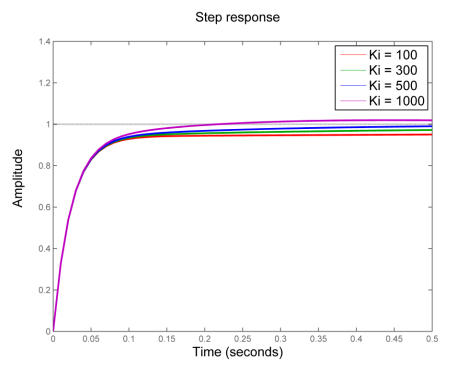
\includegraphics[width=0.5\textwidth]{billeder/pidcontrol}
\caption{PID Controller with different $K_i$ values}
\label{fig:pidcontrol}
\end{figure}
A collected table of all the effects of the three controllers can be seen in table \ref{tab:PIDcontrol}.
\begin{table}[H]
	\centering
    \begin{tabular}{|l|l|l|l|l|}
    \hline
    ~  & Rise Time    & Overshoot & Settling time & Steady-State Error \\ \hline
    $K_p$ & Decreases    & Increases & Small Change  & Decrease           \\ \hline
    $K_i$ & Decreases    & Increases & Increases     & Eliminate          \\ \hline
    $K_d$ & Small Change & Decreases & Decreases     & No Change          \\ \hline
    \end{tabular}
    \caption{PID Control effects}
    \label{tab:PIDcontrol}
\end{table}
A way to find good values for the $K_p$, $K_i$ and $K_p$ terms is to use twiddle. Twiddle or Coordinate descent works out a local minimum by doing a line search through different values of the controllers. The values can also be found in a manual way by tuning the values as you work out what is subjectively the best controller.
%------------------------------------------------
\section{SLAM}
When a robot is placed in an unknown environment, it needs to figure out where it is and how the world around it looks. For this SLAM is used, SLAM is short for Simultaneous Localization And Mapping. 
What want to achieve by using slam is to know the relative position of the robot to all seen landmarks. There is two main types of slam, online SLAM and full SLAM. online SLAM only keeps track of the relative position of the robot compared to all seen landmarks, while full SLAM keeps track of the current and all previous robot positions compared to all seen landmarks.
There are multiple SLAM algorithms, in this section, Graph SLAM will be explained shortly.

\subsection{Graph SLAM}
In the perfect world, when a robot moves, it will move exactly as intended. So if a robot is supposed to move 10 in the x direction, the new position will be $x_1 = x_0 + 10$ and $y_1 = y_0$. 
This, however is not the way it actually works. There will always be some motion noise. So instead of hitting the spot perfectly, the robot will hit the spot with some probability, which can be estimated by a Gaussian. So the new robot position will be constraint by:
\begin{equation}
f(x,y)=\frac{1}{\sqrt{2\pi\sigma^2}} \cdot e^(\frac{\frac{1}{2}(x_1-x_0-10)^2}{\sigma^2} \cdot \frac{1}{\sqrt{2\pi\sigma^2}} \cdot e^(\frac{\frac{1}{2}(y_1-y_0)^2}{\sigma^2}
\label{SLAM_eq01}
\end{equation}
This is pictured in figure \ref{SLAM_fig02}.
\begin{figure}[h!]
	\centering
    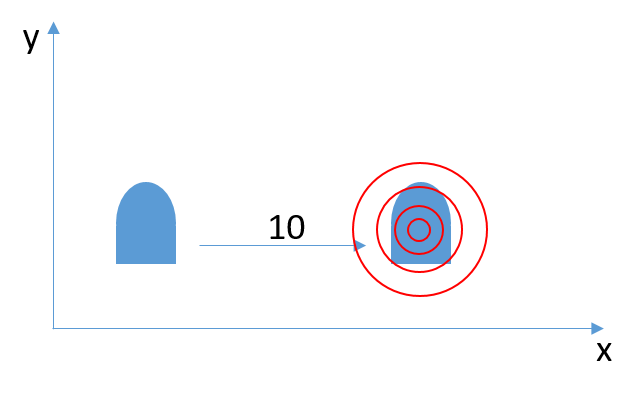
\includegraphics[scale=0.5]{billeder/GraphSLAM02.png}
    \caption{A robot in a non perfect world, moving 10 in the x direction. Noise is estimated as a Gaussian with mean $\mu = [10,0]$ and standard deviation $\sigma$.}
    \label{SLAM_fig02}
\end{figure}
What we want to do is to maximise the likelihood of the new position, given the previous position.
So what Graph SLAM does is defining the probabilities using a sequence of constraints like the one in equation \ref{SLAM_eq01}. 
If a robot moves in some space, each location is characterized by a vector that in a 2 dimensional world often is 3 dimensional (it will consist of a x-coordinate, y-coordinate and an angle). 
Graph SLAM then takes the following constraints: 
\begin{itemize}
\item \textit{Location Constraint}, which is just $x_0$.
\item \textit{Relative Motion Constraints}, which relates each robot pose to the previous robot pose. These can be seen as rubber bands.
\item \textit{Relative Measurement Constraints}, which relates each robot pose with the landmarks seen from that pose. These can also be seen as rubber bands.
\end{itemize}
Graph SLAM then relaxes the set of Relative Constraints to find the most likely configuration of a robot path along with the location of landmarks.
The way to do this is to use a quadratic matrix $\Omega$ and a vector $\xi$. $\Omega$ and $\xi$ consists of the addition of all constraints. Figure \ref{SLAM_fig04} shows an example of Graph SLAM using full SLAM. Every time a constrain is set it is added to the previous constrains. In the example, the constrains are added in the end for a better understanding of the individual steps.

\begin{figure}[H]
\centering
\begin{subfigure}{.5\textwidth}
  \centering
  
\includegraphics[width=.8\linewidth]{billeder/GraphSLAM04_1.png}
  \caption{Location Constrain}
  \label{SLAM_fig04:sub1}
\end{subfigure}%
\begin{subfigure}{.5\textwidth}
  \centering
  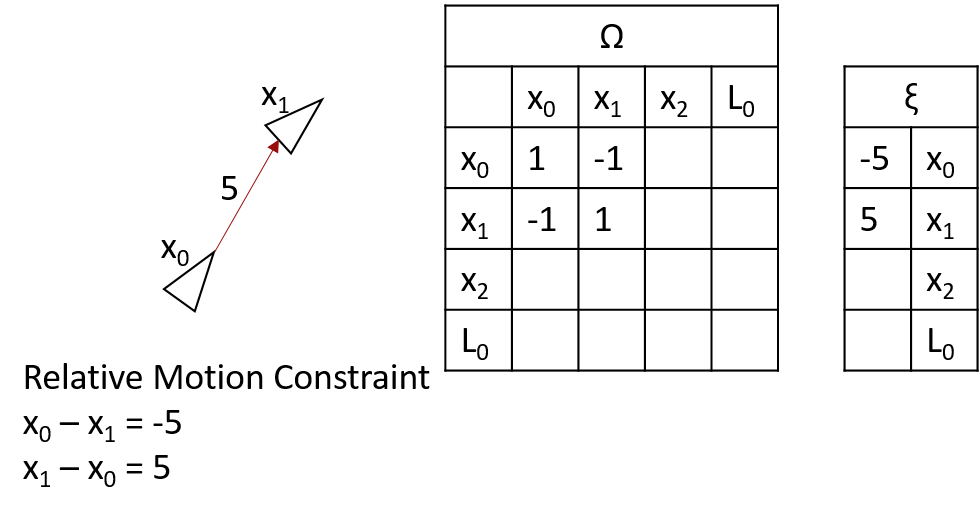
\includegraphics[width=.8\linewidth]{billeder/GraphSLAM04_2.png}
  \caption{Relative Motion Constrain from $x_0$ to $x_1$}
  \label{SLAM_fig04:sub2}
\end{subfigure}
\begin{subfigure}{.5\textwidth}
  \centering
  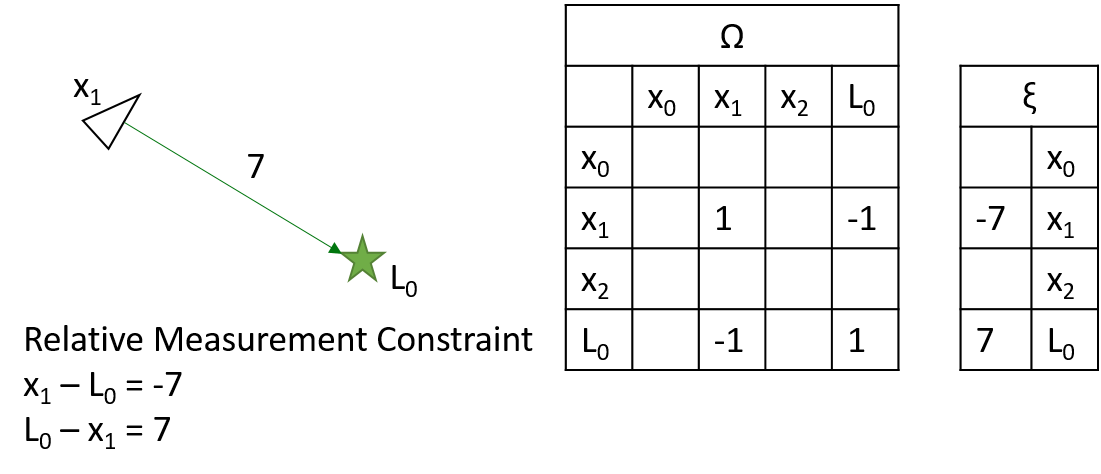
\includegraphics[width=.8\linewidth]{billeder/GraphSLAM04_3.png}
  \caption{Relative Measurement Constrain from $x_1$ to $L_0$}
  \label{SLAM_fig04:sub3}
\end{subfigure}%
\begin{subfigure}{.5\textwidth}
  \centering
  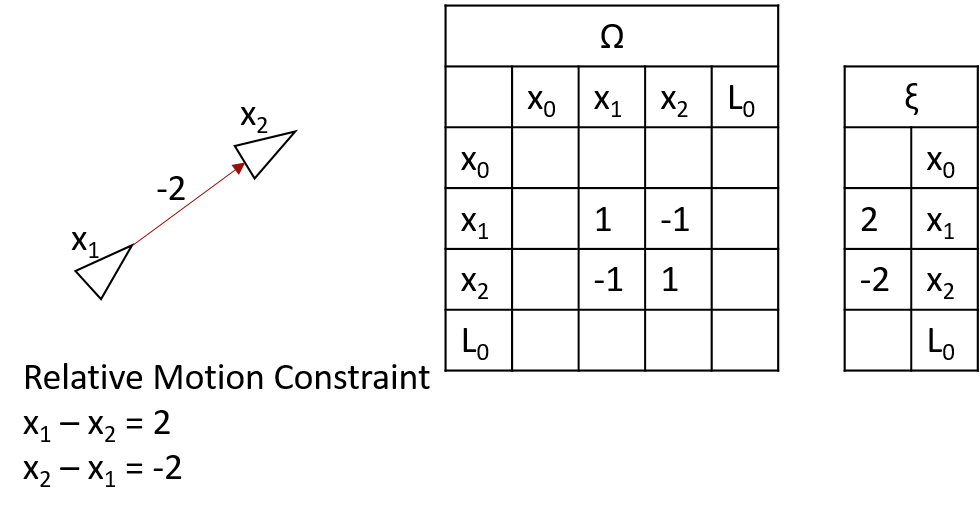
\includegraphics[width=.8\linewidth]{billeder/GraphSLAM04_4.png}
  \caption{Relative Motion Constrain from $x_1$ to $x_2$}
  \label{SLAM_fig04:sub4}
\end{subfigure}
\begin{subfigure}{.5\textwidth}
  \centering
  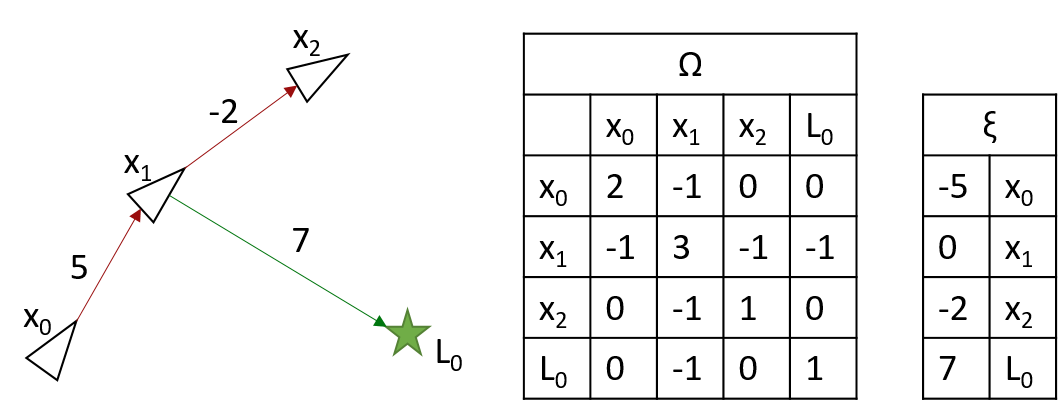
\includegraphics[width=.8\linewidth]{billeder/GraphSLAM04_5.png}
  \caption{The total Graph SLAM consists of the steps added together.}
  \label{SLAM_fig04:sub5}
\end{subfigure}
\caption{Graph SLAM illustrated.}
\label{SLAM_fig04}
\end{figure}

The most likely positions for the robot poses and the landmarks, $\mu$, are then found using equation \ref{SLAM_eq02}. 
\begin{equation}
\mu = \Omega^{-1} \cdot \xi
\label{SLAM_eq02}
\end{equation}

If noise is involved in the movements or measurements, this is handled by multiplying the constrains with $\frac{1}{\sigma}$, where $\sigma$ is the noise related to the constrain.

If the robot lives for a long time, the path taken will grow towards infinity. To avoid this, online SLAM can be used, but this will not be explained here.

%------------------------------------------------
%	Localisation
%		- Markov localisation - René
%		- Kalman - Rune
%		- Particle - Rune
%	Search and Planning - Nicolai
%	Control - Nicolai
%	SLAM - René
% chapter project
\chapter{Project}
%	Project formulation
%	Platform & Hardware
%	Design and Implementation
%		- Location
%		- Planning
%		- Driving
\section{Project formulation}
This project will entail applying knowledge from the theory chapter to create a robot capable of locating it self, and follow a path. The robot that is to be used is explained in the robot platform section.\\
Some areas of the theory is needed in order to create this system. 
These areas are localisation, path planning and movement. \\
Localisation is needed in order for the robot to locate itself within a know environment. The goal is to solve the localisation problem with a particle filter.\\
Path planning is important for the robot to be able to get to the set goal after knowing its position. The path planning problem will be solved using A\text{*}.\\
The movement will entail smoothing the path from the planner and implementing PID control to move the robot to the goal while avoiding the obstacles.\\
To properly test the implementation of these subjects, an arena will be set up with a target location and an unknown starting location. It is up to the robot to find its way home to the target location.
%\section{Platform \& Hardware}
This section contains information about the platform and hardware used in this project.


%------------------------------------------------ % Jeg tænker at alt informationen her lige så godt kunne være i design og implementation
\section{The Robot Platform}
The system is created as a simple robot that can receive move instructions, and take measurements. The move instructions come from a PC running MATLAB. By receiving the measurement data the MATLAB application calculates the best movement action, and send it to the robot. 

The overall system design can be seen in figure \ref{fig:OSD}. The connection between the Computer and the Bluetooth shield is wireless. The connection between the Bluetooth shield and the Arduino Uno is serial. The connection between the Arduino Uno and LIDAR Sensor is serial and lastly the connection between the Arduino Robot and the Arduino Uno is i2c.
\begin{figure}[H]
\centering
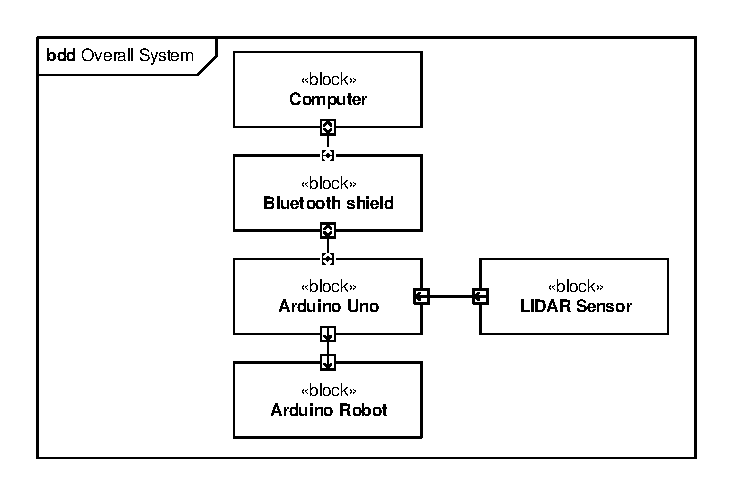
\includegraphics[width=0.7\textwidth]{billeder/OverallSystemDesign}
\caption{Overall System Design}
\label{fig:OSD}
\end{figure}
Each block in the system will now be discussed in greater detail. 

\subsubsection{Bluetooth shield}
The Bluetooth shield is an "ITEAD Wireless Bluetooth Shield Module Starter Kit For Arduino"\cite{BTshield}\cite{BTshield2}. The responsibility of the Bluetooth shield is to transfer data from the Arduino Uno to the Computer. The shield uses a HC-05 Serial Bluetooth module. Connecting to the shield is done by finding "H-C-2010-06-01" on the Computer and using the password: "1234". The settings for the serial bus is:
\begin{itemize}
\item Default baud rate: 9600
\item Data bits: 8
\item Stop bit: 1
\item No parity
\end{itemize}
This means that the Bluetooth connection can be seen as a simple uart connection between the robot and the computer. 

\subsubsection{LIDAR Sensor}
A LIDAR measurement consists of 90 packets with four range measurements in each. The packet length is 22 bytes and is organised as follows\cite{LIDAR}:
\begin{verbatim}
<start> <index> <speed_L> <speed_H> [Data 0] [Data 1] [Data 2] [Data 3]
 <checksum_L> <checksum_H>
\end{verbatim}
The $start$ code is 0xFA, $index$ goes from 0xA0 to 0xF9, $speed$ is the fixed point speed in RPM and $Data$ $N$ is the Nth reading. Each reading is four bytes in length and contains information about distance, signal strength and two flags. The data is comprised as follows:
\begin{verbatim}
<distance 7:0>  <"invalid data" flag> <"strength warning" flag> 
<distance 13:8> <signal strength 7:0> <signal strength 15:8>
\end{verbatim}
The LIDAR, also called Neato LIDAR can be seen in figure \ref{fig:NeatoLidar}.
\begin{figure}[H]
\centering
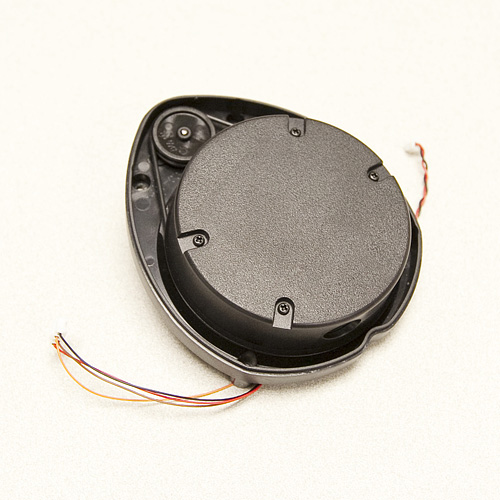
\includegraphics[scale=1]{billeder/NeatoLidar}
\caption{Neato LIDAR Sensor}
\label{fig:NeatoLidar}
\end{figure}
The LIDAR has four connects to the sensor part and two to the motor part. The motor connects are 3.3 Volt based with red being power and black being ground. The pinout for the sensor part is seen in table \ref{tab:lidars}.
\begin{table}[H]
\centering
\begin{tabular}{|l|l|}
\hline
Red & 3.3V \\ \hline
Brown & LDS\_RX \\ \hline
Orange & LDS\_TX \\ \hline
Black & GND \\ \hline
\end{tabular}
\caption{LIDAR Sensor Pinout}
\label{tab:lidars}
\end{table}
The motor is a simple DC-motor. But for a correct operation the Neato LIDAR must spin with more than 180 RPM and less than 350 RPM. The group found that a spin speed around 310 RPM gave the optimal sensor readings. This can be regulated using the speed information in the LIDAR data packets. The value in the speed bytes is formatted as RPM*64. So in order to get the RPM one must simply divide the value by 64. The group attained the optimal rotation speed, by regulating a PWM signal, on the motor. 

\subsubsection{Arduino Uno}
The Arduino Uno\cite{ArduinoUno} handles communication with the LIDAR Sensor and the Bluetooth shield.
\begin{figure}[H]
\centering
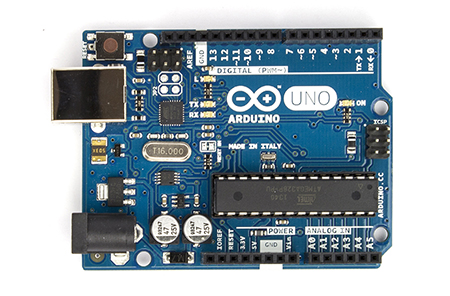
\includegraphics[scale=1]{billeder/ArduinoUno}
\caption{Arduino Uno}
\label{fig:ArduinoUno}
\end{figure}

The LIDAR data is streamed to the Arduino Uno contentiously with a baud rate on 115200. To handle the fast data rate the only hardware UART is used. The data is stored in a internal array for later retrieval.

Since there is only one hardware UART on the Arduino Uno, and both the LIDAR and the bluetooth shield needs one, a software serial port is created to handle the bluetooth communication. The Arduino Uno is listening for commands, on the bluetooth connection. A command is formatted as follows:
\begin{verbatim}
<command ID 1> <command ID 2> [Command parameters ] < 0x0A ('\n') >
\end{verbatim}
The following commands is handled by the Arduino Uno: 
\begin{tabbing}	
{LID}\={AR:}\\
\>{Comm}\={and1: <L> <D> <D/S/P/E> <\textbackslash n>} \\
\> \> D: Distance \\
\> \> S: Signal strength\\
\> \> P: Rotor speed\\
\> \> E: Error codes\\
\> Returværdi:\\
\> \> {For D og S er svaret: Array af 360 x 2 bytes big endian (Den første er altid 0 grader)} \\ \> \> {(Distance er mm)} \\
\> \> {P er en 2 byte værdi som big endian værdien er RPM*64} \\
\> \> {E er samme format som D og S, bortes fra at den kun har 360 x 1 byte} \\
\\
\> Command2: <U> <P> <\textbackslash n>\\
\> Returværdi: \\
\> \> 1 byte \= formateret som: \\
\> \> \>{[0x00] hvis ingen LIDAR data er tilgængelig.} \\
\> \> \>{[0x01] hvis LIDAR date er tilgængelig.} 

\end{tabbing}	

If any other commands is received, they are sent to the Arduino Robot over the I2C interface. 

\subsubsection{Arduino Robot}
The robot platform used in this project is a Arduino robot\cite{ArduinoRobot}. The Arduino robot platform handles all movement commands. This is done with two boards, the motor board and the control board. 
Both boards are fitted with ATmega32u4 microcontrollers. The motor board has two motors, a power bank, various communication busses, ir sensors and an on/off switch along with the microcontroller. 
The motors are of the type DC. They are controlled with a pwm signal.\\
The Control board is fitted with a speaker, external memory, various communication busses, a compass and the possibility for a LCD display.\\
When equipped with the Arduino Uno, LIDAR Sensor and the Bluetooth shield, the platform can be seen in figure \ref{fig:fullplatform}.
\begin{figure}[H]
\centering
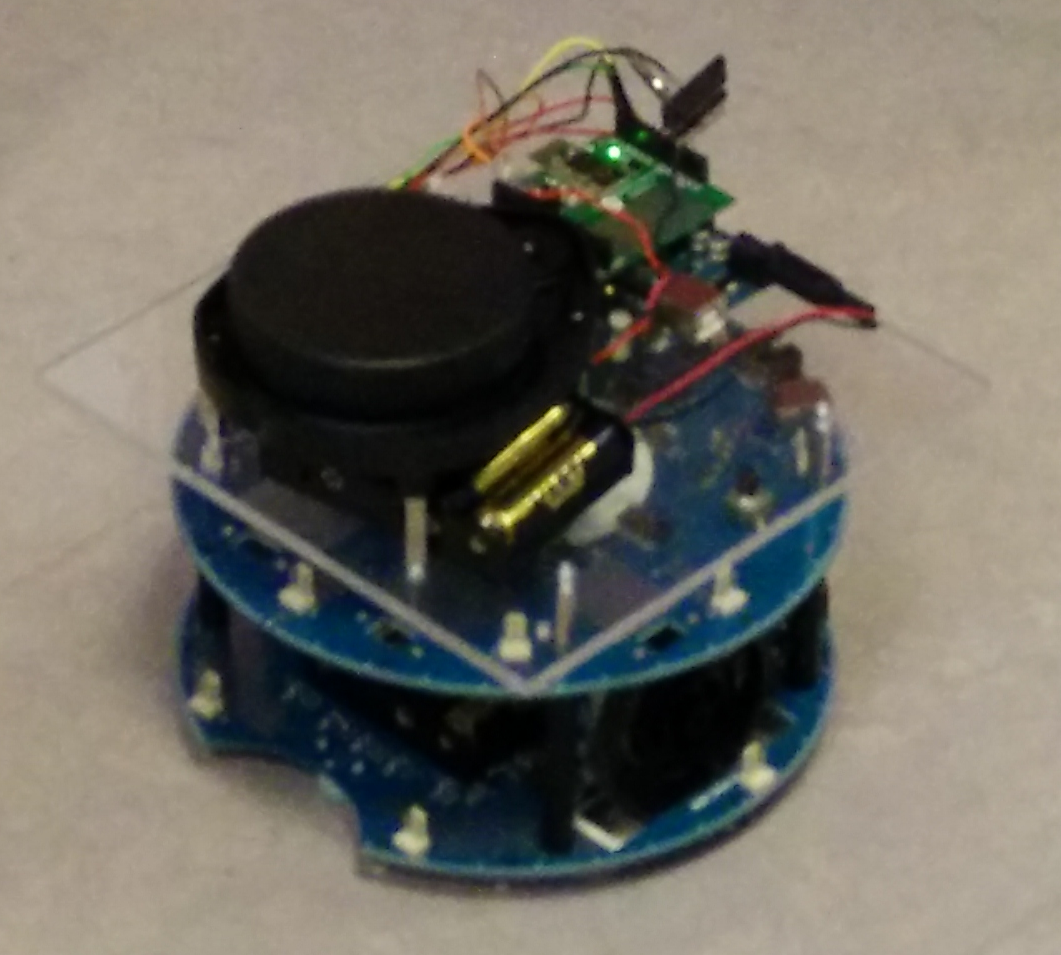
\includegraphics[width=0.6\textwidth]{billeder/fullplatform}
\caption{full platform}
\label{fig:fullplatform}
\end{figure}

The robot receives movement commands from the Arduino Uno and react on them. The Commands follows the same structure as the LIDAR commands. The Commands accepted by the robot is: 

\begin{tabbing}	
{Mot}\={or:}\\
\> {Comm}\={and: <M> <O> $[$Motor1$]$ $[$Motor2$]$ $[$Time$]$ <\textbackslash n> } \\
\> \> motor1 speed - 2 byte (-255 - 255) big endian \\
\> \> motor2 speed - 2 byte (-255 - 255) big endian\\
\> \> Time   - 2 byte big endian in ms.
\end{tabbing}	

\section{MATLAB Controller}
In this section the control actions done by the computer will be explained. The control program consists of the three sub components localisation, motion and planning. The aim of the control program is to first localize the robot. When this is achieved it must calculate a route to the desired goal, and move correctly to the goal. 

% Designandimp_Motion
\subsection{Motion}
The motion of the robot consists of two actions.
\begin{itemize}
\item Move forward 
\item Turn
\end{itemize}
Due to the lack of tachometers the robot needs an alternative way of figuring out how far it has moved or turned. The motion commands are therefore mainly based on time.

A general Move command is called by the command \textit{Move( socket, motor1, motor2, time )}, where socket is the bluetooth socket, motor1 is the speed of the right motor, motor2 is the speed of the left motor, both integer values in the range [-255:255], and time is the time in milliseconds.

\textbf{Move forward}\\
The Move forward command is called by the command \textit{[moved] = Move(obj, motor1, motor2, distance)}, where obj is the robot object, motor1 is the speed of the right motor, motor2 is the speed of the left motor, both integer values in the range [-255:255], and distance is the distance in cm. The moved parameter is the output of the Move forward command and contains the actual distance moved, based on LIDAR data.

This function consists of 2 parts. 
\begin{itemize}
\item Calculation of the time the robot must move to reach the desired distance.
\item Make sure that the robot does not bump into anything.
\end{itemize}
To find the time it takes for the robot to move, a measurement was made. The robot was placed behind a line, and different times were given to the function. The distance the robot travelled was then measured. In the end a function was fitted to the curve, and this function is the basic of the Move function.

\begin{figure}[H]
\centering
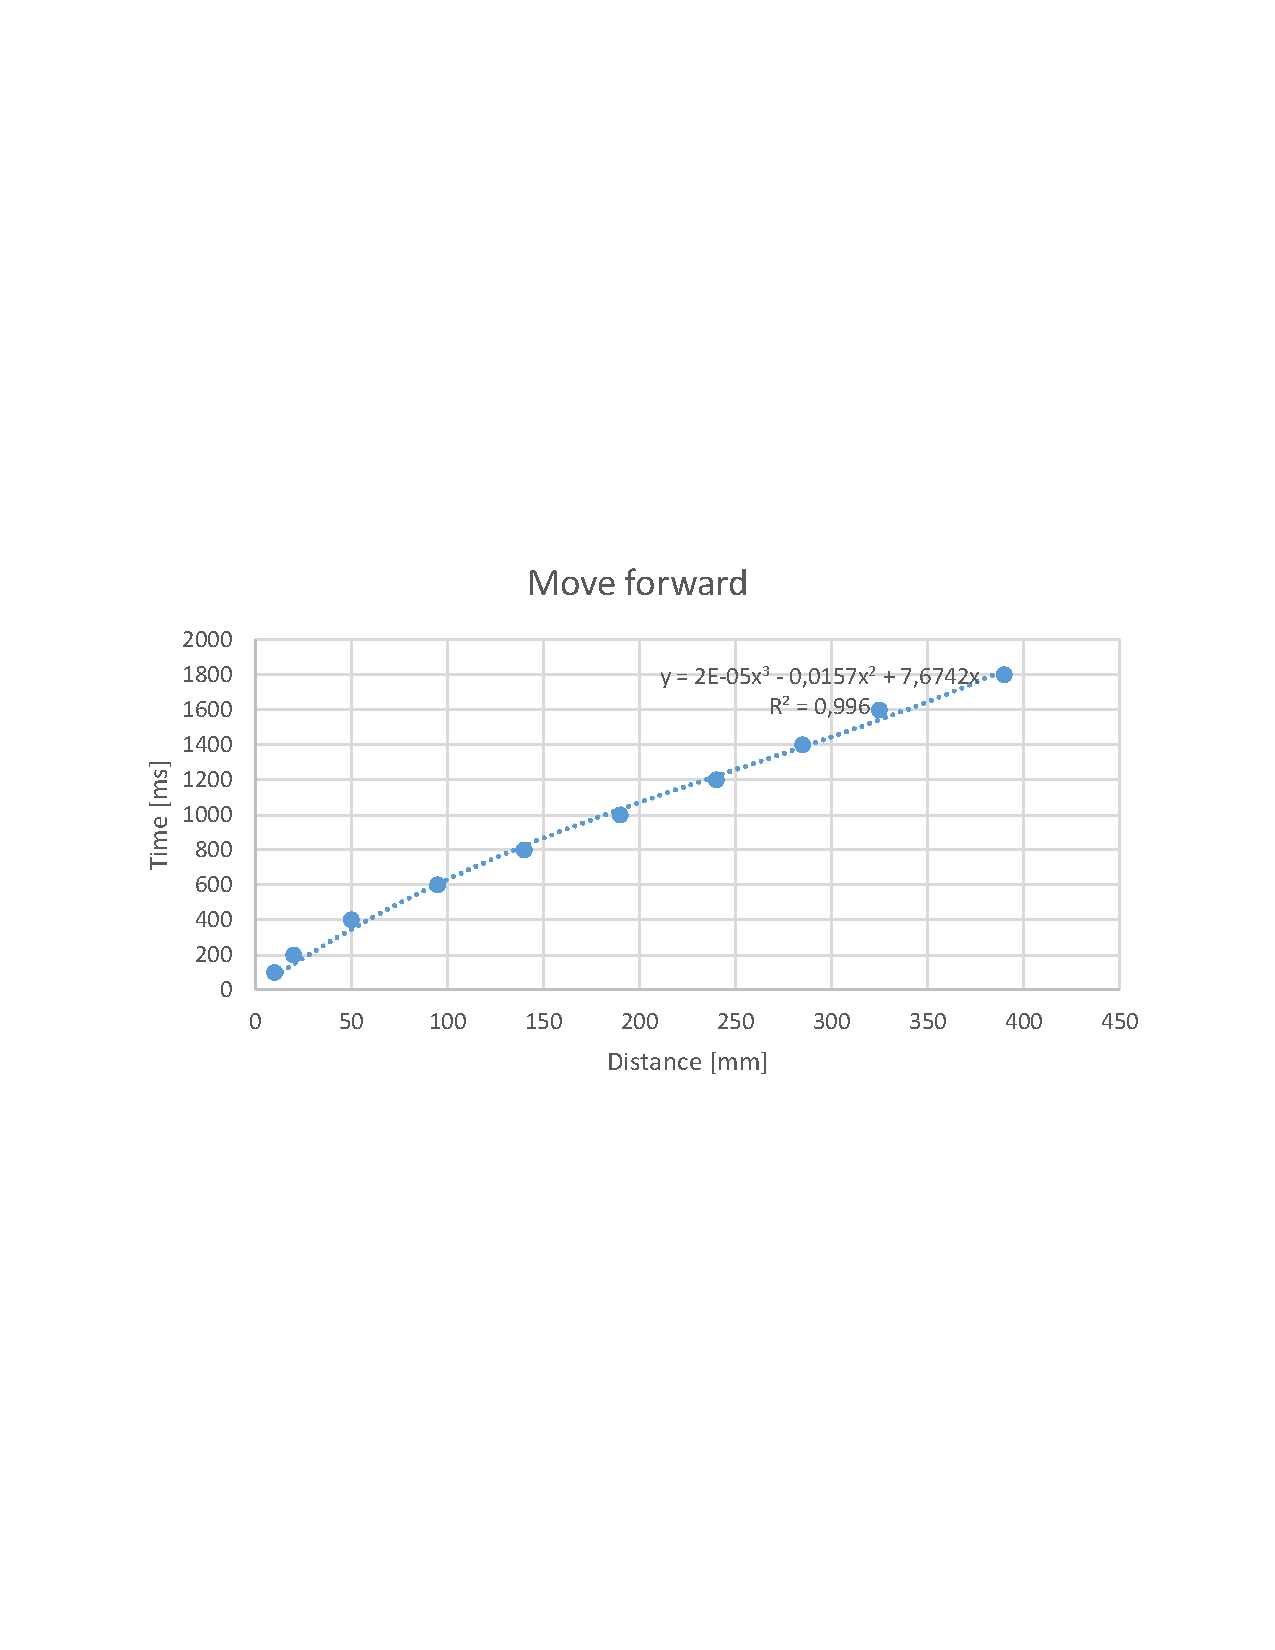
\includegraphics[width=0.8\textwidth]{billeder/MoveForwardGraph.pdf}
\caption{Measurement of Move forward}\label{MoveForwardGraph}
\end{figure} 

The main problem is that when the robot is using up battery, it does not move as far in the same given time as when it is fully charged. Therefore a measurement is made with the LIDAR before and after the movement to get a better fit of how far the robot actually moved. The measurement takes account of failing measurements, so that if the measurement straight ahead fails, it will use the nearest angle instead. The two distances is then calculated using trigonometry.
The difference between the two distances is the actual movement of the robot, and it is this value that is returned from the function.
The reason why LIDAR is not used directly to move a specific distance is the update rate of the LIDAR data. It is simply too slow. The function then calls the general Move command with the calculated time.

Despite the fact that the LIDAR has a slow update rate, it is used as a safe distance detection. If an object is detected in the area shown in figure \ref{MotionBumper}, the robot stops its movement and the function returns the moved distance. Due to the slow update rate of the LIDAR, the safe distance is relatively high. In the project, the forward safety distance is set to 250 mm. and the safety distance to each side is 200 mm.

\begin{figure}[H]
\centering
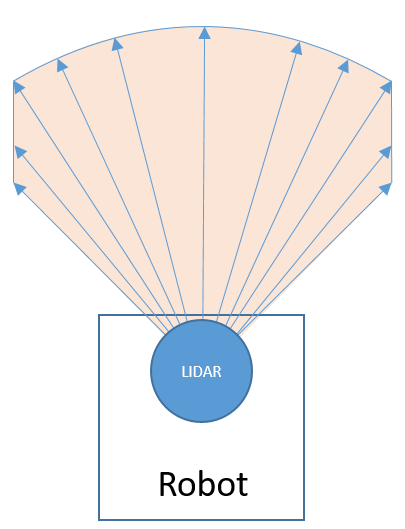
\includegraphics[scale=0.7]{billeder/MotionBumper.png}
\caption{Area of bump detection. The robot is facing up.}\label{MotionBumper}
\end{figure} 

\textbf{Turn}\\
The Turn command is called by the command \textit{Turn(obj, phi)}, where obj is the robot object and phi is the turning angle in degrees. The range of phi is [-180:180] with decimals accepted. This function calculates the time it will take for the robot to turn to the angle received, and calls the general Move function with one motor in reverse and the other in forward position. 
To get a way to calculate the time, a measurement similar to the on for the Move forward function was made. The robot was placed at a point and a mark was made where it had its 0 degrees. Then the general move function was called with different times and the angle the robot turned was measured. Figure \ref{TurnRightGraph} and \ref{TurnLeftGraph} shows the result of the measurements.

\begin{figure}[H]
\centering
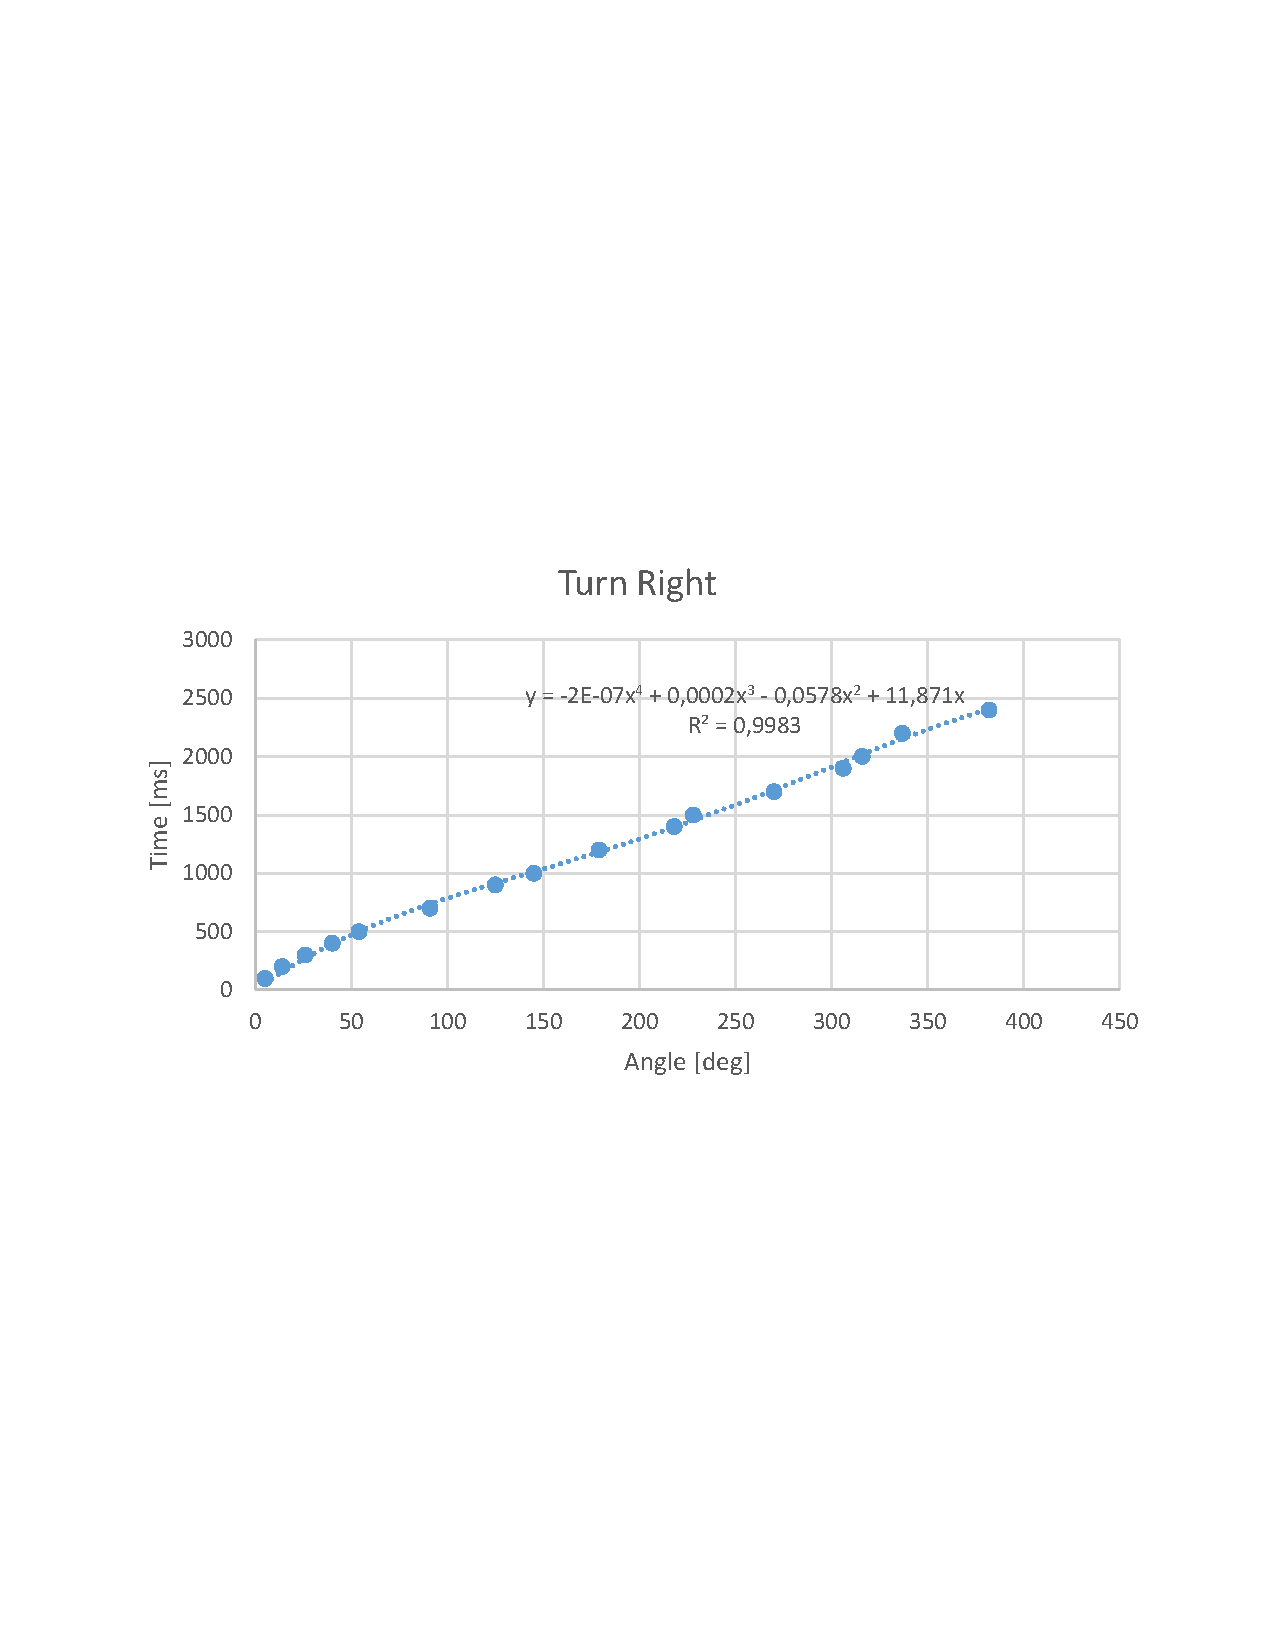
\includegraphics[width=0.8\textwidth]{billeder/TurnRightGraph.pdf}
\caption{Measurement of Turn right}\label{TurnRightGraph}
\end{figure} 
\begin{figure}[H]
\centering
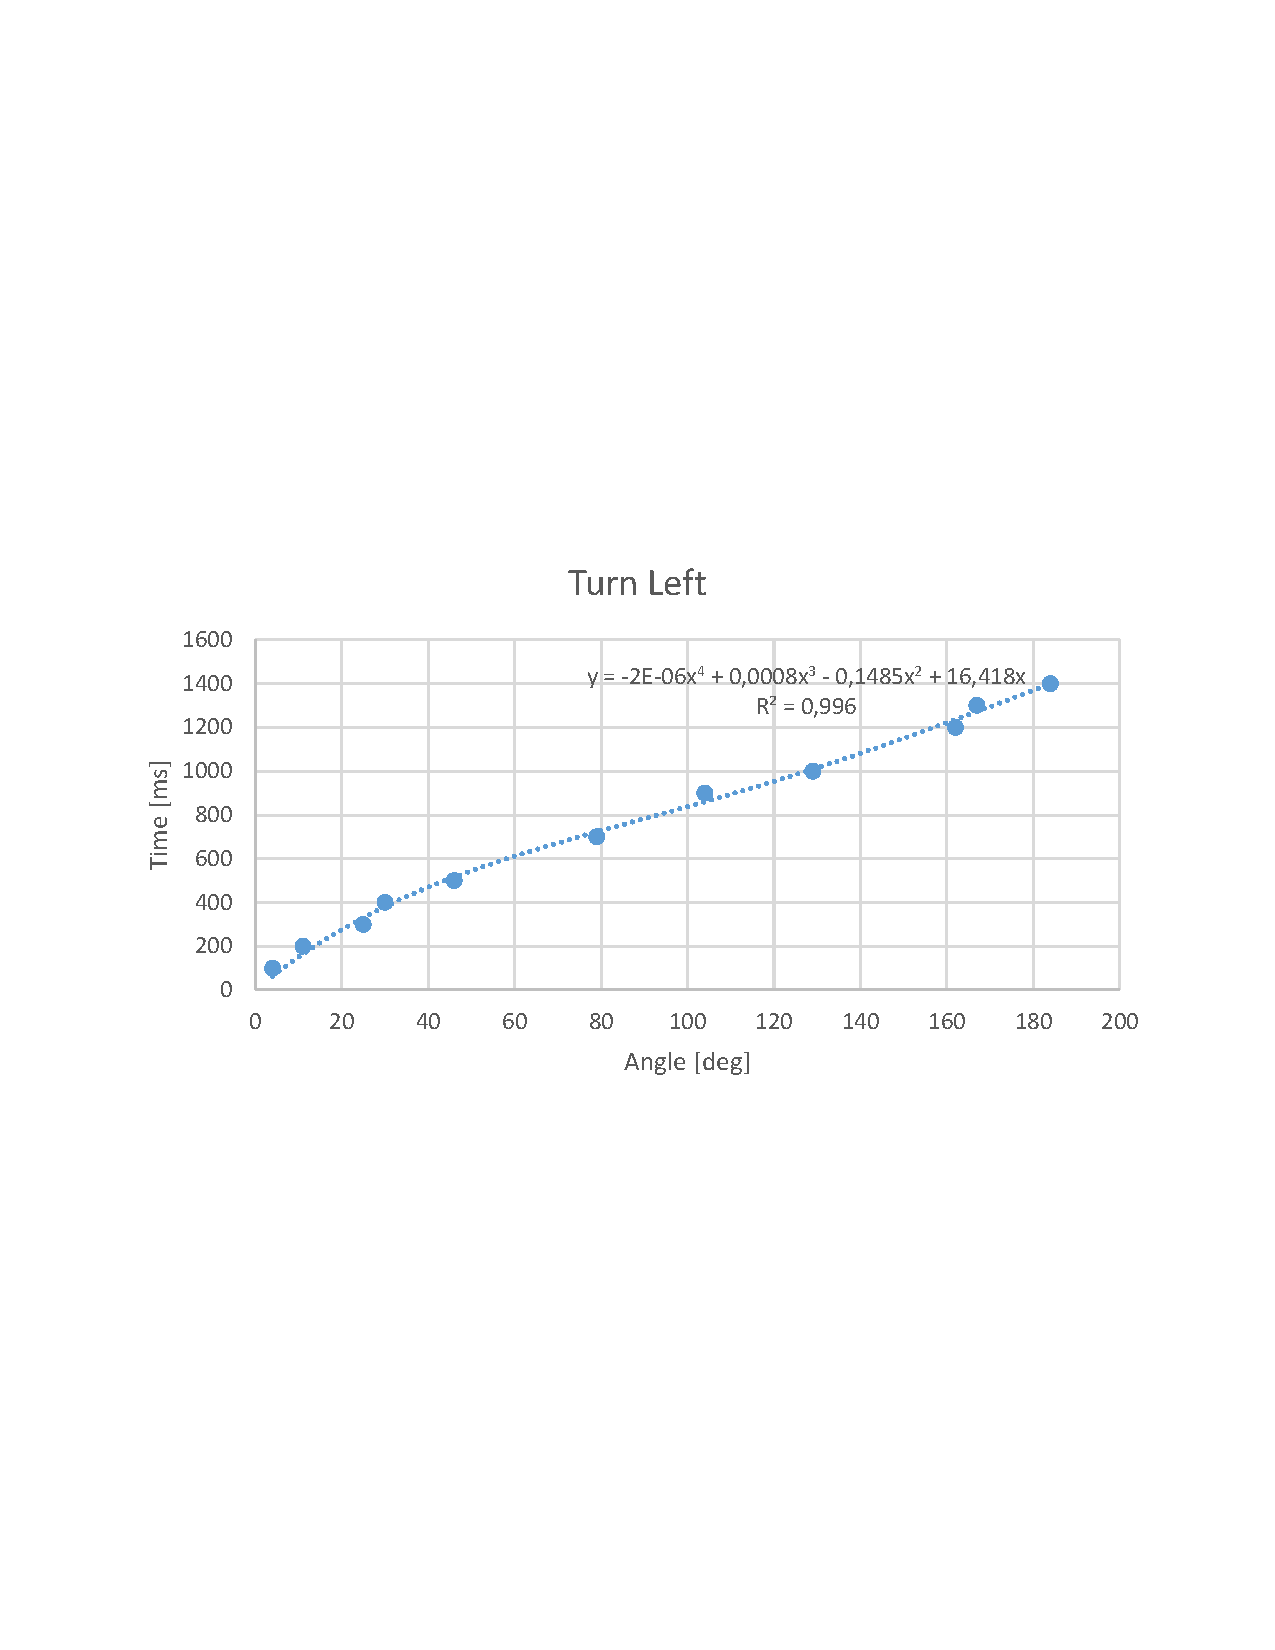
\includegraphics[width=0.8\textwidth]{billeder/TurnLeftGraph.pdf}
\caption{Measurement of Turn left}\label{TurnLeftGraph}
\end{figure} 

The same problem with the battery power arises in this function. Therefore a scanning is made by the LIDAR before the turn is performed. After the turn is made, the LIDAR scans again and the robot compares the two measurements by convolution. Then it starts to step one degree until a maximum in the convolution is found. This is then expected to be a more correct guess of the desired angle.


\subsection{Localisation Using Particle Filter}
In order to localize the robot a particle filter was used. The filter works by following a series of steps. 

\textbf{Step 1: Initialize the filter}\\
First 200 particles was created and given a random position and orientation on the map. In MATLAB this is simply a big 3x200 matrix with $[x, y, phi]$ for each of the 200 particles. 

\textbf{Step 2: Getting The Robot Measurement}\\
At this step we get the robot measurement. But even though all 360 measurements would give a very precise filter, the time it will take calculate the particle distances in 360 degrease would be too long. In this project we have chosen to use 20 measurements, but less can in theory be used. The less measurements that are used in the filter, the bigger the risk of getting symmetric error locations. These locations will die over time, but for a system with too few measurements it can take quiet a while. 

The data from the robot is a series of distances and angels. If we plot this for our robot it can look like shown on figure \ref{RobotData}.

\begin{figure}[H]
\centering
\begin{subfigure}{.5\textwidth}
  \centering
  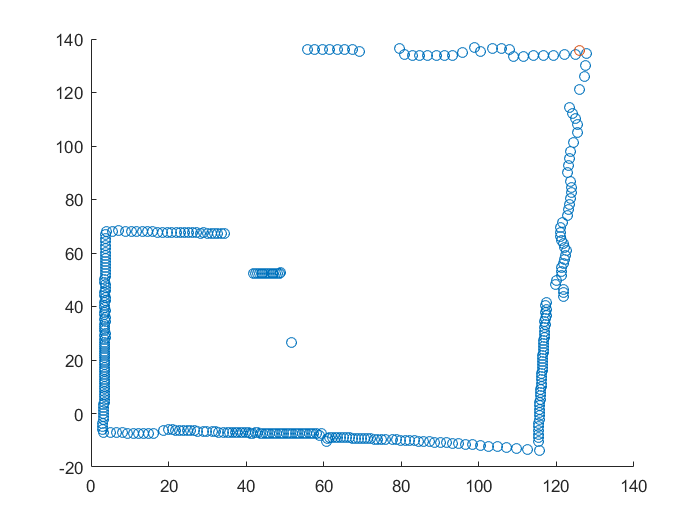
\includegraphics[width=1.2\linewidth]{billeder/SeeData.png}
  \label{ResultDriveFig1:sub1}
\end{subfigure}%
\begin{subfigure}{.5\textwidth}
  \centering
  \includegraphics[width=.6\linewidth]{billeder/Results/real3.png}
  \label{ResultDriveFig1:sub2}
\end{subfigure}
\caption{Robot LIDAR Data}
\label{RobotData}
\end{figure}

As seen on the figure there is a gap in the readings where the black pillar is at the top of the image. This is a area where the LIDAR is not able to read. This introduces another problem if we compare a error reading with a particle correct reading. This can give a good particle a bad probability later on.
To fix this we start taking only the good readings, and then take 20 measurements equally spaced from the set. We now have a set with 20 distances and what angle they where measured in. 

\textbf{Step 3: Getting The Particle Measurement}\\
Now the particles measurements at the same angles as the real robots measurements must be found. We have done this by a ray casting technique where we put a point at the particle position. Then we move the point a little bit in the beam direction and check if there is a obstacle. If this is not the case we move the point a little more. We continue this process till we hit a obstacle.\\
This is done for all particles in all measurement directions. When the algorithm is done the result is a 20x200 matrix containing all measurements for all particles. 

\textbf{Step 4: Calculating Particle probability}\\

By comparing each particles measurements to the real robots measurements the probability for how likely it is that the real robot have the same position and orientation as the particle is calculated. This is done using equation \ref{EQProb}. 

\begin{equation}
	Prob(P_{dis},R_{dis})= e^{-{\frac{(P_{dis_1} - R_{dis_1})^2}{2 \cdot Noise^2}}} \cdot e^{-{\frac{(P_{dis_2} - R_{dis_2})^2}{2 \cdot Noise^2}}} \cdot ... \cdot e^{-{\frac{(P_{dis_{20}} - R_{dis_{20}})^2}{2 \cdot Noise^2}}}
\label{EQProb}
\end{equation}

A important factor here is the noise that indicates how mush a particle and the real robots measurements can differ, and still be a good fit. The noise must be set fairly high since we also what particle close to the true value to survive, and not just the ones on the true value. 

\textbf{Step 5: Finding The Best Fit}\\
At some point we need to decide where the robot is, according to the particle information. There is many approaches that can be used to decide this. Some look at the mean value, others look at clusters. In our implementation we took a simple approach and took the particle with the highest probability and selected as our guess on the robot location. 

\textbf{Step 6: Resample Or Reset}\\
Now it is time to do the resampling of the particles. This only make sense if there is atleast one good estimate since a resampling basically focuses the filter around the best guesses. If all guesses are bad, it will focus around random bad guesses. To counter effect this we made the filter restart and go back to step 1 if the best guess is under 10\% certainty. By doing this we force the filter to reset if it have no clue where the robot is. 

\textbf{Step 7: Move the robot}\\
In order to get a better estimate more information must be given to the filter. This can only be achieved if the robot moves. When the robot does not know where it is it can simply move randomly around. To simplify this behaviour we have made the robot move in the longest free direction it can see with the LIDAR. 

If the robot have a good guess on its location at this point it moves towards the next point in its movement plan. The movement plan is created the first time the robot get a guess on its location that is over 70\% certainty and is from that point on followed, unless the filter gets reset. The movement plan is the route calculated using A* from the robot location, found by the filter, to the desired goal. 

\textbf{Step 8: Updating the filter}\\
The filter is now updated by moving and turning all the particles the same amount as the real robot just did. In addition to the move, all particles are also moved and turn a little bit at random. This is to simulate the effect of the noise in the robot movement. After this step we go back to step 2 and continues from there in a never ending loop. 

After a few iterations the filter will collect all particles in a small cloud around the robot position. The width and height of the cloud is detriment by the movement noise, and the noise in particle probability equation. Finding good values for the noise model is critical for a well functioning filter. In our small project fixed values was used that was found over a process of trail and error.  Similar values could be found by creating a noise model for the robot and LIDAR. In more advanced implementations it is also common to use a adaptive approach changing the values on the fly. 
\subsubsection{Path Planning}
The path planning consist of two actions, finding a path with A\text{*} and then calculating coordinate targets in the map. 
A\text{*} uses a know map, an initial position, the goal and a cost map to plan out the path to the goal. 
The internal functionality of the A\text{*} function generates a heuristic map based on the goal and the know map. The implementation of A\text{*} is based upon the implementation from the Artificial Intelligence in Robotics Udacity course\citep{AIROK}.\\
The output of the A\text{*} is a path and a policy vector. The policy vector is used to calculate some coordinate targets which are used as targets when the robot moves towards the goal. An example of a plan can be seen in figure \ref{fig:exastar} where start is [ 1 1 ] and the goal is [ 6 5 ]. For a real world example see the results section.
\begin{figure}[H]
\centering
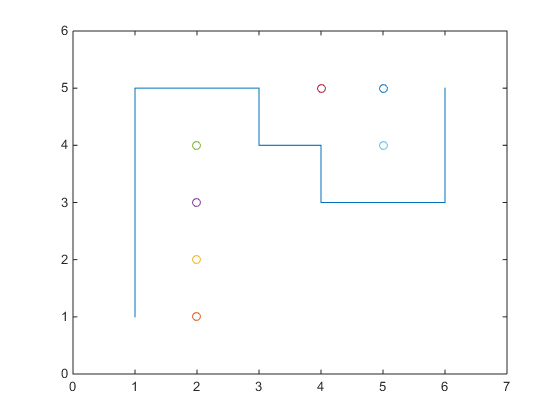
\includegraphics[width=0.5\textwidth]{billeder/exampleastar}
\caption{Example of A star plan}
\label{fig:exastar}
\end{figure}
 
%------------------------------------------------
\section{Results}
Here the results, of a run in the test arena with a random initial position and a goal in [20, 120], will be shown.
Figure \ref{ResultDriveFig1} shows how the robot initially tries to find its own location, using the particle filter. The number of particles is 200. It drives towards the farthest point read by the LIDAR while analysing its surroundings. In figure \ref{ResultDriveFig1:sub5} we see that the probability of a particle is over the threshold of 70\%, so the robots starts to plan its way towards the goal, using A*. 
\begin{figure}[H]
\centering
\begin{subfigure}{.5\textwidth}
  \centering
  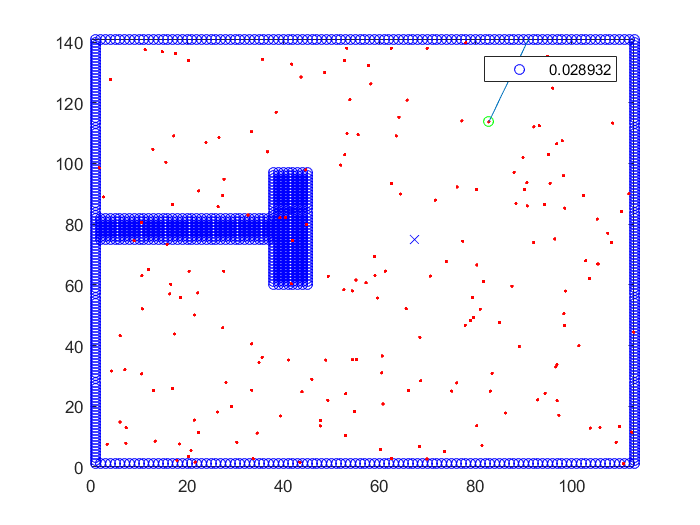
\includegraphics[width=.8\linewidth]{billeder/Results/1.png}
  \caption{Step 1}
  \label{ResultDriveFig1:sub1}
\end{subfigure}%
\begin{subfigure}{.5\textwidth}
  \centering
  \includegraphics[width=.7\linewidth]{billeder/Results/real1.png}
  \caption{Step 1}
  \label{ResultDriveFig1:sub2}
\end{subfigure}
\begin{subfigure}{.5\textwidth}
  \centering
  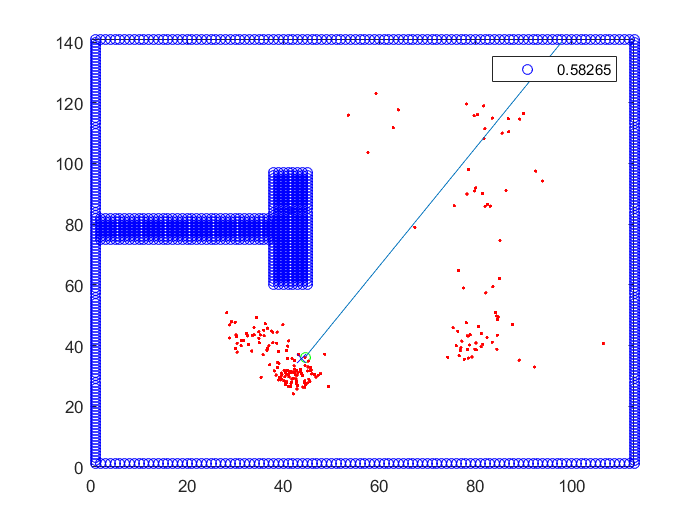
\includegraphics[width=.8\linewidth]{billeder/Results/3.png}
  \caption{Step 3}
  \label{ResultDriveFig1:sub3}
\end{subfigure}%
\begin{subfigure}{.5\textwidth}
  \centering
  \includegraphics[width=.7\linewidth]{billeder/Results/real3.png}
  \caption{Step 3}
  \label{ResultDriveFig1:sub4}
\end{subfigure}
\begin{subfigure}{.5\textwidth}
  \centering
  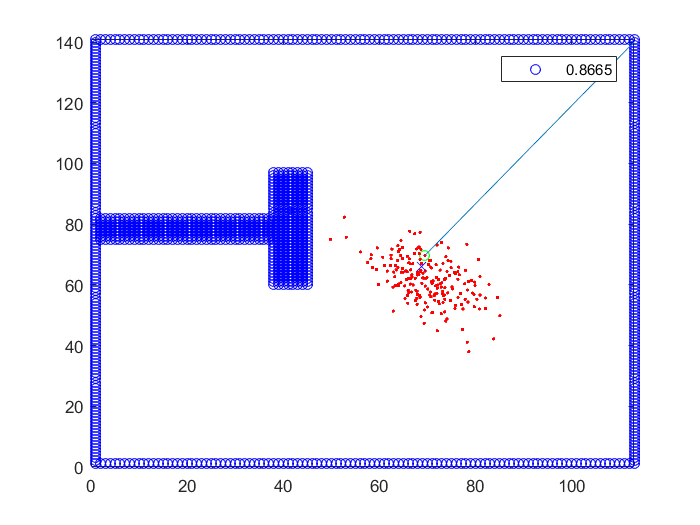
\includegraphics[width=.8\linewidth]{billeder/Results/5.png}
  \caption{Step 5}
  \label{ResultDriveFig1:sub5}
\end{subfigure}%
\begin{subfigure}{.5\textwidth}
  \centering
  \includegraphics[width=.7\linewidth]{billeder/Results/real5.png}
  \caption{Step 5}
  \label{ResultDriveFig1:sub6}
\end{subfigure}
\caption{The robot tries to find its location.}
\label{ResultDriveFig1}
\end{figure}
Figure \ref{ResultDriveFig2} shows the robot trying to make it towards the points of the plan. The point the robot is aiming for is marked by a blue '+' on the particle filter map. The robot has to be within  5 cm of the point to believe that it is in the correct position.
\begin{figure}[H]
\centering
\begin{subfigure}{.5\textwidth}
  \centering
  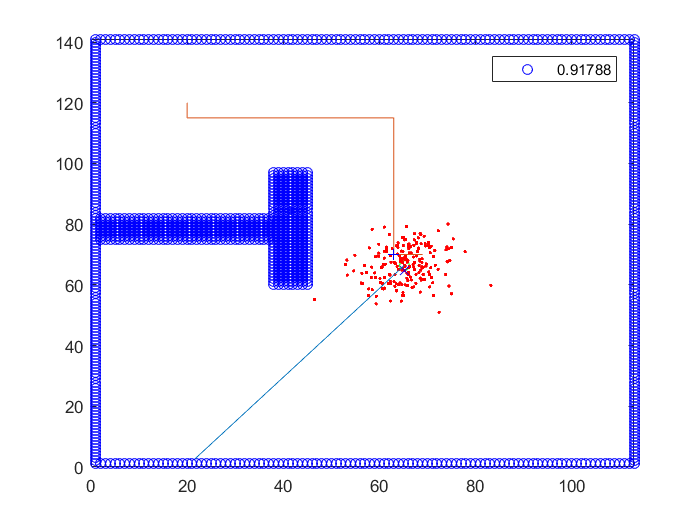
\includegraphics[width=.8\linewidth]{billeder/Results/7.png}
  \caption{Step 7}
  \label{ResultDriveFig2:sub1}
\end{subfigure}%
\begin{subfigure}{.5\textwidth}
  \centering
  \includegraphics[width=.7\linewidth]{billeder/Results/real7.png}
  \caption{Step 7}
  \label{ResultDriveFig2:sub2}
\end{subfigure}
\begin{subfigure}{.5\textwidth}
  \centering
  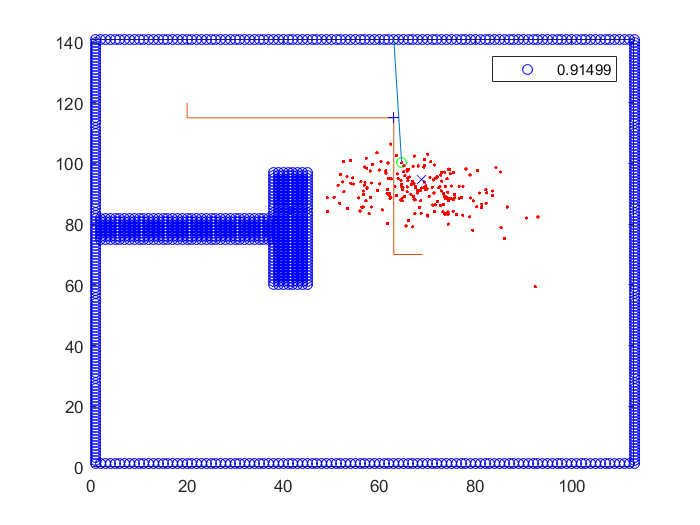
\includegraphics[width=.8\linewidth]{billeder/Results/9.png}
  \caption{Step 9}
  \label{ResultDriveFig2:sub3}
\end{subfigure}%
\begin{subfigure}{.5\textwidth}
  \centering
  \includegraphics[width=.7\linewidth]{billeder/Results/real9.png}
  \caption{Step 9}
  \label{ResultDriveFig2:sub4}
\end{subfigure}
\begin{subfigure}{.5\textwidth}
  \centering
  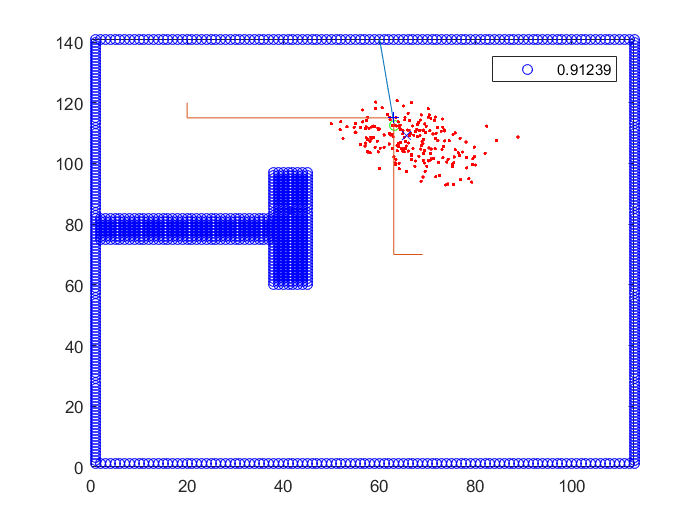
\includegraphics[width=.8\linewidth]{billeder/Results/11.png}
  \caption{Step 11}
  \label{ResultDriveFig2:sub5}
\end{subfigure}%
\begin{subfigure}{.5\textwidth}
  \centering
  \includegraphics[width=.7\linewidth]{billeder/Results/real11.png}
  \caption{Step 11}
  \label{ResultDriveFig2:sub6}
\end{subfigure}
\caption{The robot makes a map and moves along the points on the path.}
\label{ResultDriveFig2}
\end{figure}

\begin{figure}[H]
\centering
\begin{subfigure}{.5\textwidth}
  \centering
  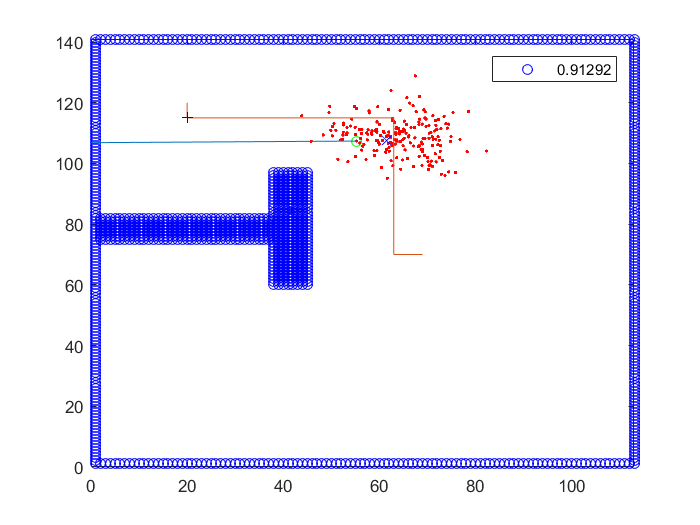
\includegraphics[width=.8\linewidth]{billeder/Results/13.png}
  \caption{Step 13}
  \label{ResultDriveFig3:sub1}
\end{subfigure}%
\begin{subfigure}{.5\textwidth}
  \centering
  \includegraphics[width=.7\linewidth]{billeder/Results/real13.png}
  \caption{Step 13}
  \label{ResultDriveFig3:sub2}
\end{subfigure}
\begin{subfigure}{.5\textwidth}
  \centering
  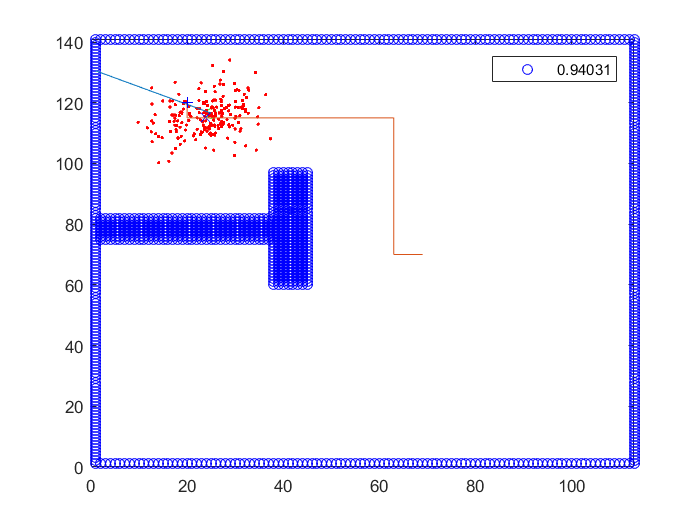
\includegraphics[width=.8\linewidth]{billeder/Results/19.png}
  \caption{Step 19}
  \label{ResultDriveFig3:sub3}
\end{subfigure}%
\begin{subfigure}{.5\textwidth}
  \centering
  \includegraphics[width=.7\linewidth]{billeder/Results/real19.png}
  \caption{Step 19}
  \label{ResultDriveFig3:sub4}
\end{subfigure}
\begin{subfigure}{.5\textwidth}
  \centering
  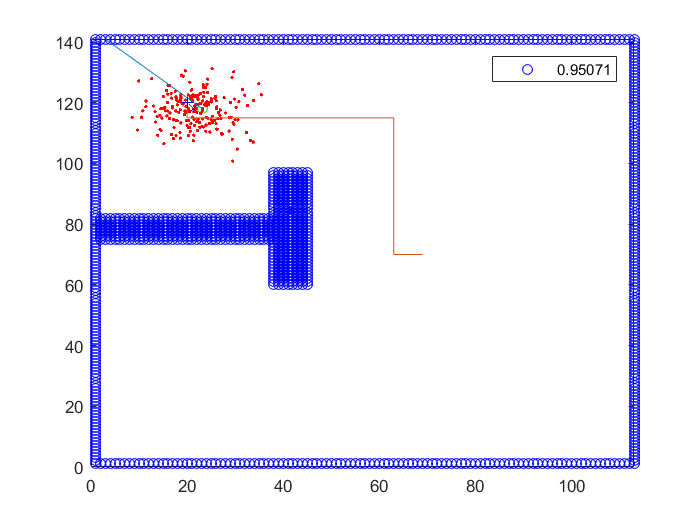
\includegraphics[width=.8\linewidth]{billeder/Results/23.png}
  \caption{Step 23}
  \label{ResultDriveFig3:sub5}
\end{subfigure}%
\begin{subfigure}{.5\textwidth}
  \centering
  \includegraphics[width=.7\linewidth]{billeder/Results/real23.png}
  \caption{Step 23}
  \label{ResultDriveFig3:sub6}
\end{subfigure}
\caption{The robot moves along the last points of the path and reaches goal.}
\label{ResultDriveFig3}
\end{figure}

The robot used 3 steps to find it self and in total it took 23 steps from beginning to end. 

%------------------------------------------------
\chapter{Discussion}
The motors were not fitted with tachometers which meant there was no way of getting reliable information about the wheels movement. This made it hard to determine the distance driven and the drift to either side. As a direct consequence of this, PID control and path smoothing was not used as the implementation of the PID controller would have been very complex and only relying on measurements from the LIDAR sensor. It was chosen that the PID controller implementation was out of the scope of this project. \\
To try to correct some of the movement noise the LIDAR data was used to inform of the actual movement. This worked fairly well for us. If we had more time one interesting experiment would be to use a Kalman filter to fuse the measurement from the LIDAR with the time based control input to get a even better estimate.

When a path plan is made, the plan is made from single centimetre steps into a  few coordinate sets. 
This is done because the robot has a hard time following the line and because of the lack of information from the wheels. 
When the robot is sufficiently close to one of the coordinate points, it will turn and head towards the next.
From the result it can be seen that the robot uses a lot of steps to achieve its goal after the correct path is found. 
This is mainly because the robot is not very certain of its own position, since most steps happens when it tries to get close to the point.

Another problem that was often seen during the previous testing, was that the robot drifted to one side. This was somewhat solved by giving one motor a slightly higher speed than the other. The drifting error became higher the longer the robot drove in one step. Therefore the maximal distance to drive was also set to 30 cm. This gives the robot a higher precision in movements, but it also results in more movements when longer routes are planned.\\
The Move forward function was not corrected the same way as the Turn function was. If it was corrected directly by reversing, if the robot drove too far, some of the overshoots may have been avoided.

When using the particle filter it is important to set the noise values corrected to get a optimal filter. In our filter the noise settings was good for finding the area where the true location was with relative few particles. But the noise settings prevented us for tuning in on the true location, by decreasing the area. This could be achieved by changing the noise as a function of the certainty.   
Another important aspect to consider when working with particle filters is the number of particles to be used. For a large map many particles is needed. The more particles the greater the calculation cost. It is therefore sometimes better to decrease the number of particles when the location have been found, since the very large amount is only truly needed in the initial location state. The optimal number is dependent of the application.

Some considerations shall also be made in regards to the re-sample time. In our implementation we re-sampled after every move. But for some applications it is a better strategy to make a series of moves and see how the probability of the particles is over time and re-sample based on this information. It is shown when comparing our results to results made by a other group, that this strategy preforms better in situations with many symmetric locations. This is since the re-sample operation is way more costly than the move operation. When doing a series of movements the chance of leaving the symmetric area before a re-sampling increases. 


\chapter{Conclusion}


%----------------------------------------------------------------------------------------
%	REFERENCE LIST
%----------------------------------------------------------------------------------------

\begingroup
	\raggedright
	\bibliography{bibtex/litteratur}							% Litteraturlisten inkluderes
\endgroup

%----------------------------------------------------------------------------------------

%\end{multicols}

\end{document}